\documentclass[12pt,a4paper]{article}

% Codificacion e idioma
\usepackage[T1]{fontenc}
\usepackage[utf8]{inputenc}
\usepackage[spanish,es-nodecimaldot]{babel}
\usepackage{lmodern}
\usepackage{microtype}

% Pagina y tipografia
\usepackage[a4paper,margin=2.5cm]{geometry}
\usepackage{setspace}
\onehalfspacing
\usepackage{fancyhdr}
\usepackage{titlesec}

% Tablas, figuras y color
\usepackage{graphicx}
\graphicspath{{figures/eda/}{figures/d1/}{figures/d2/}{figures/d3/}{figures/d4/}{figures/d5/}{figures/d6/}}
\usepackage{booktabs}
\usepackage{tabularx}
\usepackage{longtable}
\usepackage{array}
% Compatibilidad entre la versión local de array y columnas p{} usadas por tabularx.
\makeatletter
\providecommand{\insert@pcolumn}{\insert@column}
\makeatother
\usepackage{enumitem}
\usepackage{float}
\usepackage[font=small,labelfont=bf,justification=centering]{caption}
\usepackage{subcaption}
\usepackage[table]{xcolor}

% Matematica y codigo
\usepackage{amsmath,amssymb,mathtools}
\usepackage{listings}
\lstset{basicstyle=\ttfamily\small,breaklines=true,frame=single,language=Python,showstringspaces=false}

% Enlaces, referencias y bibliografia
\usepackage{csquotes}
\usepackage[backend=biber,style=apa,sorting=nyt]{biblatex}
\addbibresource{references.bib}
\usepackage[colorlinks=true,linkcolor=blue,citecolor=blue,urlcolor=blue]{hyperref}
\usepackage[nameinlink,capitalise,noabbrev]{cleveref}

% Encabezados y secciones
\pagestyle{fancy}
\fancyhf{}
\lhead{\ProyectoTitulo}
\rhead{EVA1}
\cfoot{\thepage}
\setlength{\headheight}{14.5pt}
\titleformat{\section}{\Large\bfseries}{\thesection.}{0.6em}{}
\titleformat{\subsection}{\large\bfseries}{\thesubsection.}{0.6em}{}
\setlist[itemize]{leftmargin=*,noitemsep,topsep=0.4em}
\renewcommand{\arraystretch}{1.18}

\newcommand{\ProyectoTitulo}{Evaluación de Factibilidad del Proyecto Heart Disease}
\newcommand{\ProyectoSubtitulo}{Gestión de Proyectos de Datos --- EVA1}
\newcommand{\ProyectoAutor}{Lucas Moncada \quad Ignacio Silva \quad Fabián Leal \quad Vicente Hormazábal \quad César Rojas}
\newcommand{\ProyectoFecha}{Noviembre de 2026}

\title{\ProyectoTitulo\\[0.4em]\large \ProyectoSubtitulo}
\author{\ProyectoAutor}
\date{\ProyectoFecha}

% Comandos reutilizables para el documento.
\newcommand{\TODO}[1]{\textcolor{red}{\textbf{TODO:} #1}}
\newcommand{\figref}[1]{\cref{#1}}
\newcommand{\tabref}[1]{\cref{#1}}

\renewcommand{\ProyectoTitulo}{Documentación técnica del modelo Heart Disease}
\renewcommand{\ProyectoSubtitulo}{Datos, preparación, entrenamiento y evaluación experimental}
\renewcommand{\ProyectoFecha}{Noviembre de 2026}

\begin{document}
\hypersetup{pageanchor=false}
\begin{titlepage}
  \centering
  \vspace*{2.2cm}
  {\Large Duoc UC\par}
  \vspace{2.0cm}
  {\Huge\bfseries Documentación técnica del modelo Heart Disease\par}
  \vspace{0.8cm}
  {\Large Datos, preparación, entrenamiento y evaluación experimental\par}
  \vspace{1.5cm}
  {\large Gestión de Proyectos de Datos --- EVA1\par}
  \vfill
  {\large Lucas Moncada \quad Ignacio Silva \quad Fabián Leal\par}
  {\large Vicente Hormazábal \quad César Rojas\par}
  \vspace{0.8cm}
  {\large Noviembre de 2026\par}
\end{titlepage}
\hypersetup{pageanchor=true}
\pagenumbering{roman}
\tableofcontents
\clearpage
\pagenumbering{arabic}

\section{Propósito y alcance}
Este documento describe exclusivamente el prototipo académico de clasificación construido con el archivo \texttt{heart.csv}: composición de los datos, auditoría, transformaciones, entrenamiento, selección, evaluación y artefactos reproducibles. No describe un sistema clínico desplegado. El modelo no está validado en población local chilena y no debe usarse para diagnóstico, tratamiento, priorización asistencial ni decisiones sobre pacientes.

La implementación reproducible está en \texttt{notebooks/04\_implementacion\_tecnica\_3\_1\_2.ipynb} y \texttt{src/modeling.py}. La fuente académica se conserva en \texttt{data/raw/heart.csv}; el entrenamiento elimina duplicados exactos en memoria y no modifica el original.

\section{Dataset y variables}
El archivo contiene 1.025 filas, 13 predictores y la variable binaria \texttt{target}; se observan 723 filas duplicadas exactas y 302 filas únicas. No se detectaron valores nulos. La etiqueta se conserva como está codificada en el archivo; su significado y su equivalencia clínica no se dan por validados para una población distinta.

\begin{table}[H]
  \centering
  \caption{Diccionario resumido de variables}
  \label{tab:diccionario-datos}
  \scriptsize
  \resizebox{\textwidth}{!}{%
  \begin{tabular}{lllll}
    \toprule
    Variable & Descripción & Tipo & Unidad / codificación & Dominio observado \\
    \midrule
    age & Edad del paciente. & Numérica discreta & años & 29--77 \\
    sex & Sexo del paciente. & Binaria & 0=mujer; 1=hombre & 0|1 \\
    cp & Tipo de dolor torácico. & Categórica & No verificada; ver CSV & 0|1|2|3 \\
    trestbps & Presión arterial en reposo al ingreso. & Numérica discreta & mmHg & 94--200 \\
    chol & Colesterol sérico. & Numérica discreta & mg/dL & 126--564 \\
    fbs & Indicador de glucosa en ayunas superior a 120 mg/dL. & Binaria & 0=no; 1=sí (>120 mg/dL) & 0|1 \\
    restecg & Resultado del electrocardiograma en reposo. & Categórica & 0=normal; 1=ST-T; 2=HVI & 0|1|2 \\
    \bottomrule
  \end{tabular}%
  }
\end{table}

\begin{table}[H]
  \centering
  \caption{Diccionario resumido de variables (continuación)}
  \label{tab:diccionario-datos-cont}
  \scriptsize
  \resizebox{\textwidth}{!}{%
  \begin{tabular}{lllll}
    \toprule
    Variable & Descripción & Tipo & Unidad / codificación & Dominio observado \\
    \midrule
    thalach & Frecuencia cardíaca máxima alcanzada. & Numérica discreta & bpm & 71--202 \\
    exang & Angina inducida por ejercicio. & Binaria & 0=no; 1=sí & 0|1 \\
    oldpeak & Depresión del segmento ST inducida por ejercicio respecto del reposo. & Numérica continua & desviación ST & 0--6.2 \\
    slope & Pendiente del segmento ST durante ejercicio. & Categórica & No verificada; ver CSV & 0|1|2 \\
    ca & Número de vasos principales coloreados por fluoroscopia. & Numérica discreta & UCI: 0--3; CSV: 0--4 & 0--4 \\
    thal & Resultado de la prueba de talio. & Categórica & No verificada; ver CSV & 0|1|2|3 \\
    target & Variable objetivo binaria de la versión Kaggle, asociada a la presencia de enfermedad cardíaca. & Binaria & Binaria 0/1; ver CSV & 0|1 \\
    \bottomrule
  \end{tabular}%
  }
\end{table}


Las variables numéricas usadas como cuantitativas por el pipeline son \texttt{age}, \texttt{trestbps}, \texttt{chol}, \texttt{thalach} y \texttt{oldpeak}. Se codifican como categóricas \texttt{sex}, \texttt{cp}, \texttt{fbs}, \texttt{restecg}, \texttt{exang}, \texttt{slope}, \texttt{ca} y \texttt{thal}. Aunque algunas variables binarias o de conteo están almacenadas como enteros, su tipo estadístico y su tratamiento del modelo no se infieren sólo del dtype.

La copia presenta diferencias de dominio con la documentación de UCI, en particular para \texttt{cp}, \texttt{slope}, \texttt{ca} y \texttt{thal}. El caso \texttt{ca=4} se conserva como observado. No se inventa una recodificación semántica cuando la versión concreta del dataset no permite sostenerla \parencite{uci-heart-disease,kaggle-heart}.

\section{Auditoría y preparación de datos}
\subsection{Duplicados, nulos y dominios}
Se detectaron 723 duplicados exactos al comparar las 14 columnas. El flujo conserva las 302 observaciones distintas y deduplica antes de particionar para impedir que copias idénticas queden simultáneamente en entrenamiento y prueba. También verifica combinaciones repetidas de predictores con etiquetas en conflicto; no se encontraron casos. No hay identificador de paciente, por lo que no se puede determinar si las repeticiones son publicaciones repetidas o mediciones de una misma persona.

No se observaron nulos, de modo que no se imputa. El pipeline valida columnas esperadas, clases binarias de \texttt{target} y ausencia de nulos. Los dominios categóricos observados se preservan y se contrastan con la ficha de la fuente; las categorías nuevas se rechazan en la rutina batch y no se asignan silenciosamente.

\begin{figure}[H]
  \centering
  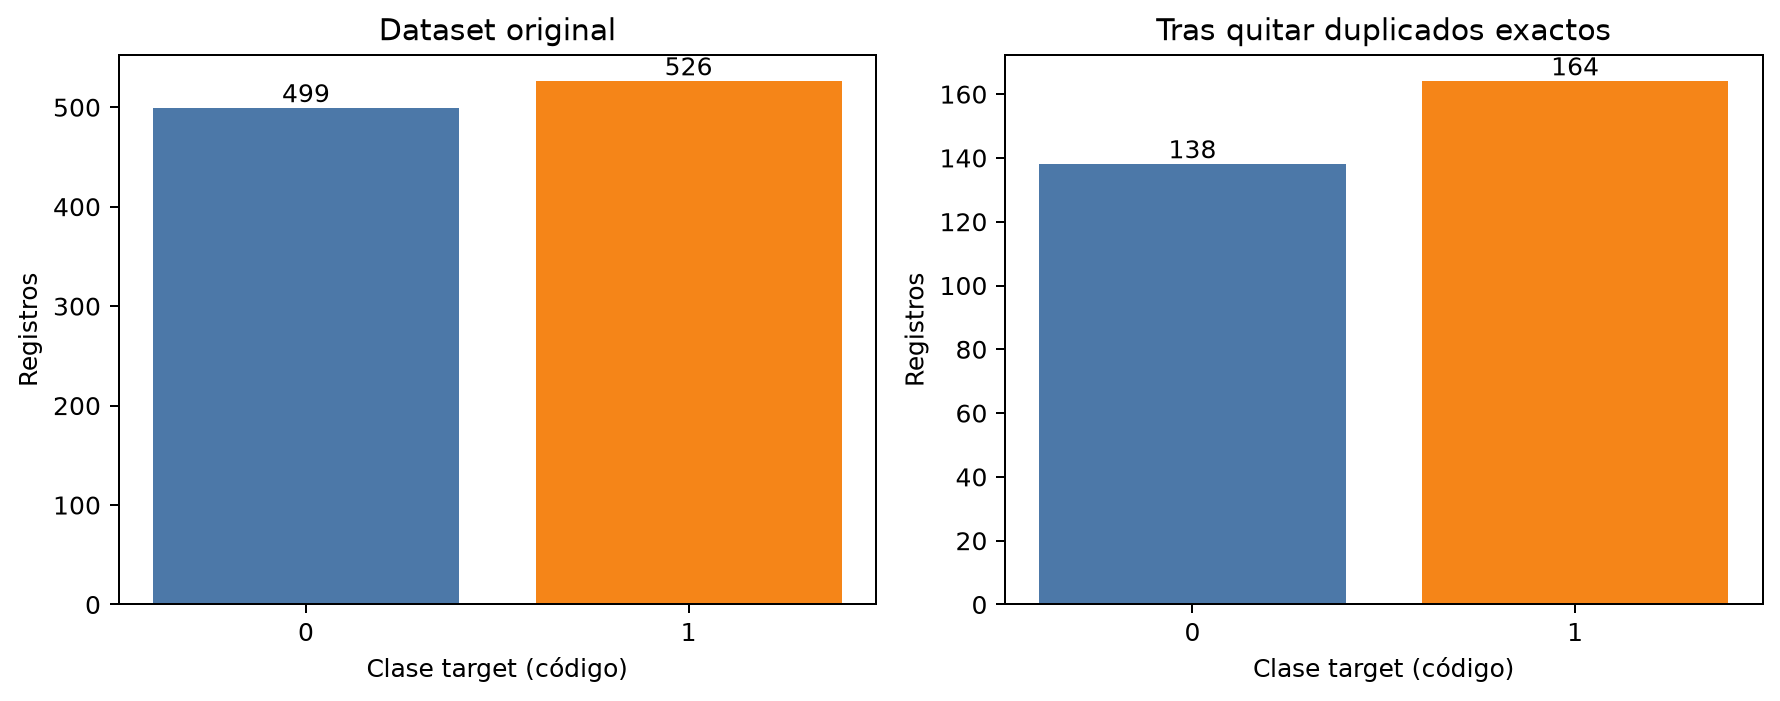
\includegraphics[width=0.88\textwidth]{../outputs/figures/distribucion_clases_antes_despues_deduplicar.png}
  \caption{Distribución de clases antes y después de quitar duplicados exactos. La deduplicación cambia el peso relativo de las clases, por lo que se aplica antes de separar los datos.}
  \label{fig:clases}
\end{figure}

\subsection{Extremos y escalado}
La regla exploratoria de 1,5 veces el rango intercuartílico marca 9 valores de \texttt{trestbps}, 5 de \texttt{chol}, 1 de \texttt{thalach} y 5 de \texttt{oldpeak}; no marca valores de \texttt{age}. Se conservan: la regla señala casos para revisar, pero no demuestra que sean errores. No se aplicó recorte ni winsorización.

No se aplica una normalización uniforme a todos los algoritmos. La regresión logística de referencia usa \texttt{RobustScaler} en las variables cuantitativas y one-hot en las categóricas. XGBoost recibe las cuantitativas en escala original y las categóricas one-hot, porque el modelo de árboles divide mediante umbrales y no requiere estandarización como la regresión logística. Los transformadores se ajustan dentro de cada pipeline/fold, evitando que estadísticas del conjunto de prueba entren en el preprocesamiento.

\begin{figure}[H]
  \centering
  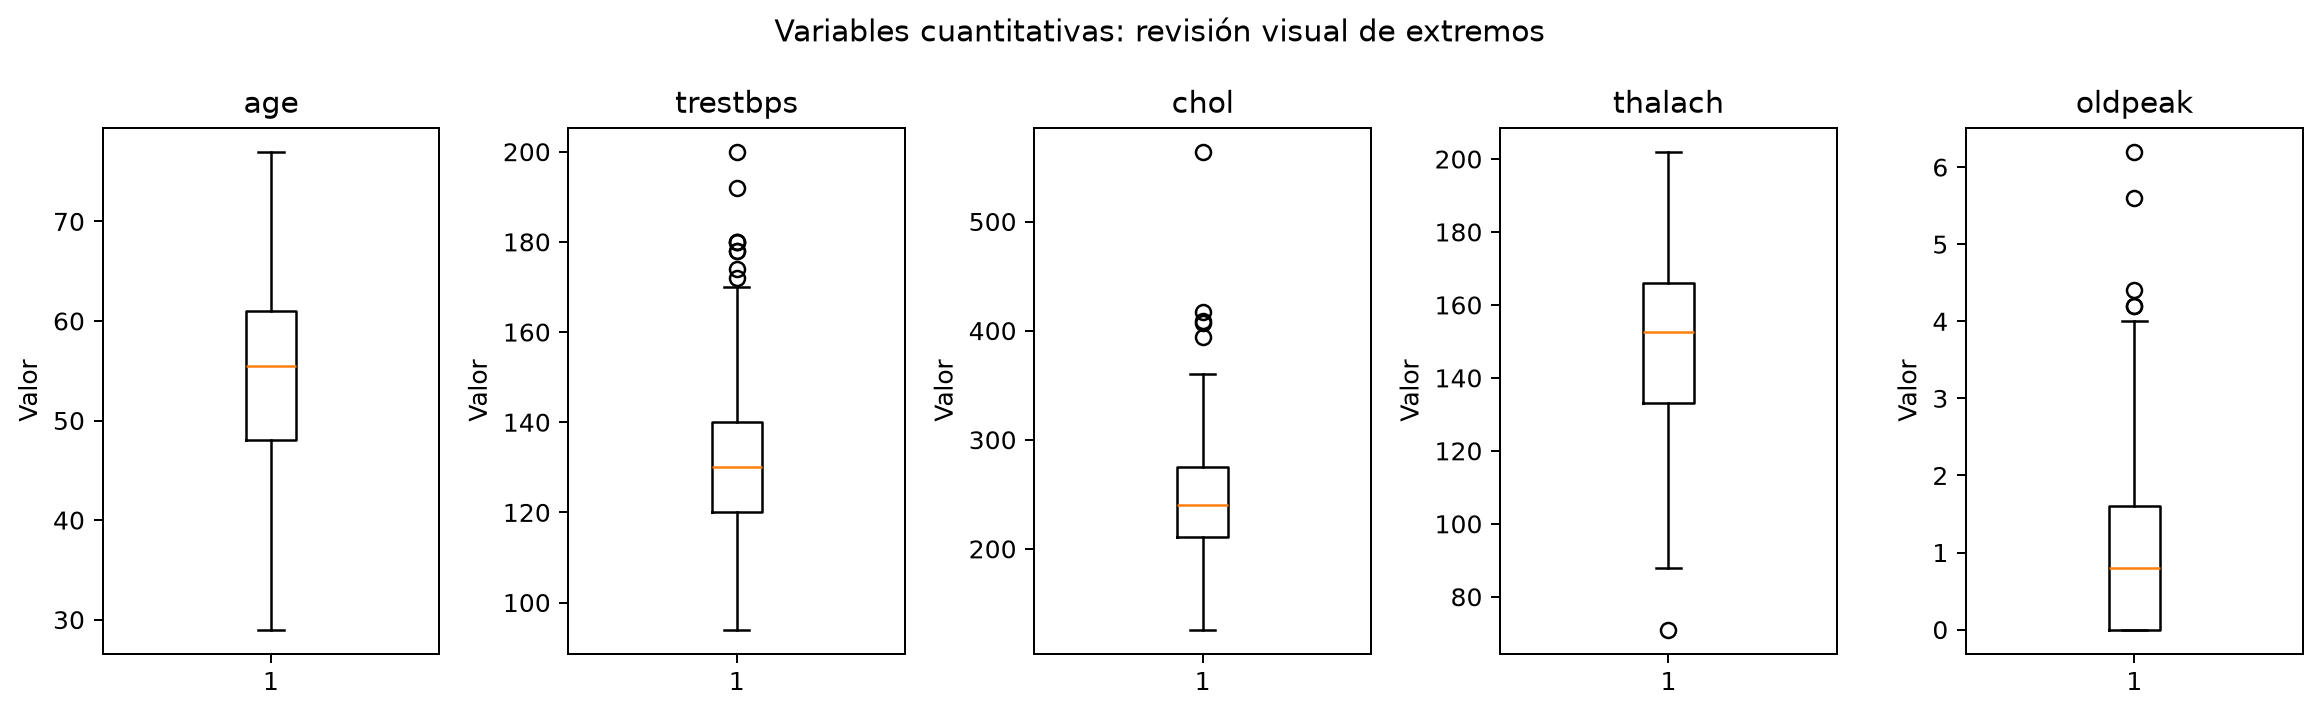
\includegraphics[width=0.93\textwidth]{../outputs/figures/diagramas_caja_variables_cuantitativas.png}
  \caption{Distribuciones de variables cuantitativas y candidatos a revisión según el criterio IQR.}
  \label{fig:iqr}
\end{figure}

\section{Relaciones exploratorias}
La correlación de Pearson se calcula entre variables cuantitativas y la etiqueta binaria. Para variables categóricas se representa por separado la correlación de cada indicador de nivel con \texttt{target}. Estos gráficos describen asociaciones en esta muestra; no muestran causalidad ni bastan para excluir predictores. Los códigos categóricos no se interpretan como magnitudes continuas.

\begin{figure}[H]
  \centering
  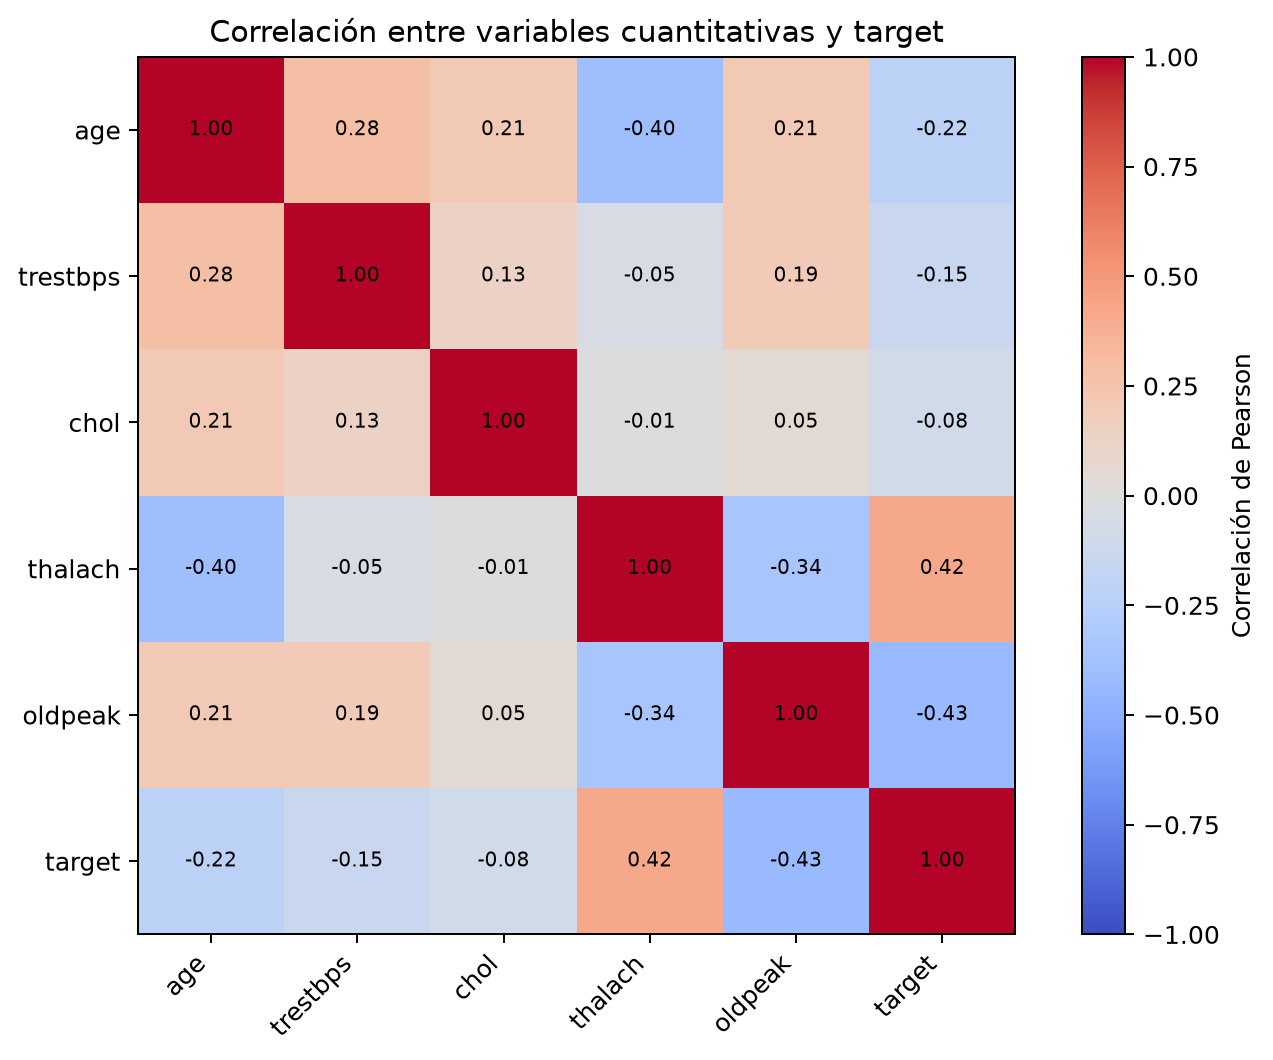
\includegraphics[width=0.91\textwidth]{../outputs/figures/matriz_correlacion_continuas_target.png}
  \caption{Correlación de Pearson de predictores cuantitativos y \texttt{target}.}
  \label{fig:corr-num}
\end{figure}

\begin{figure}[H]
  \centering
  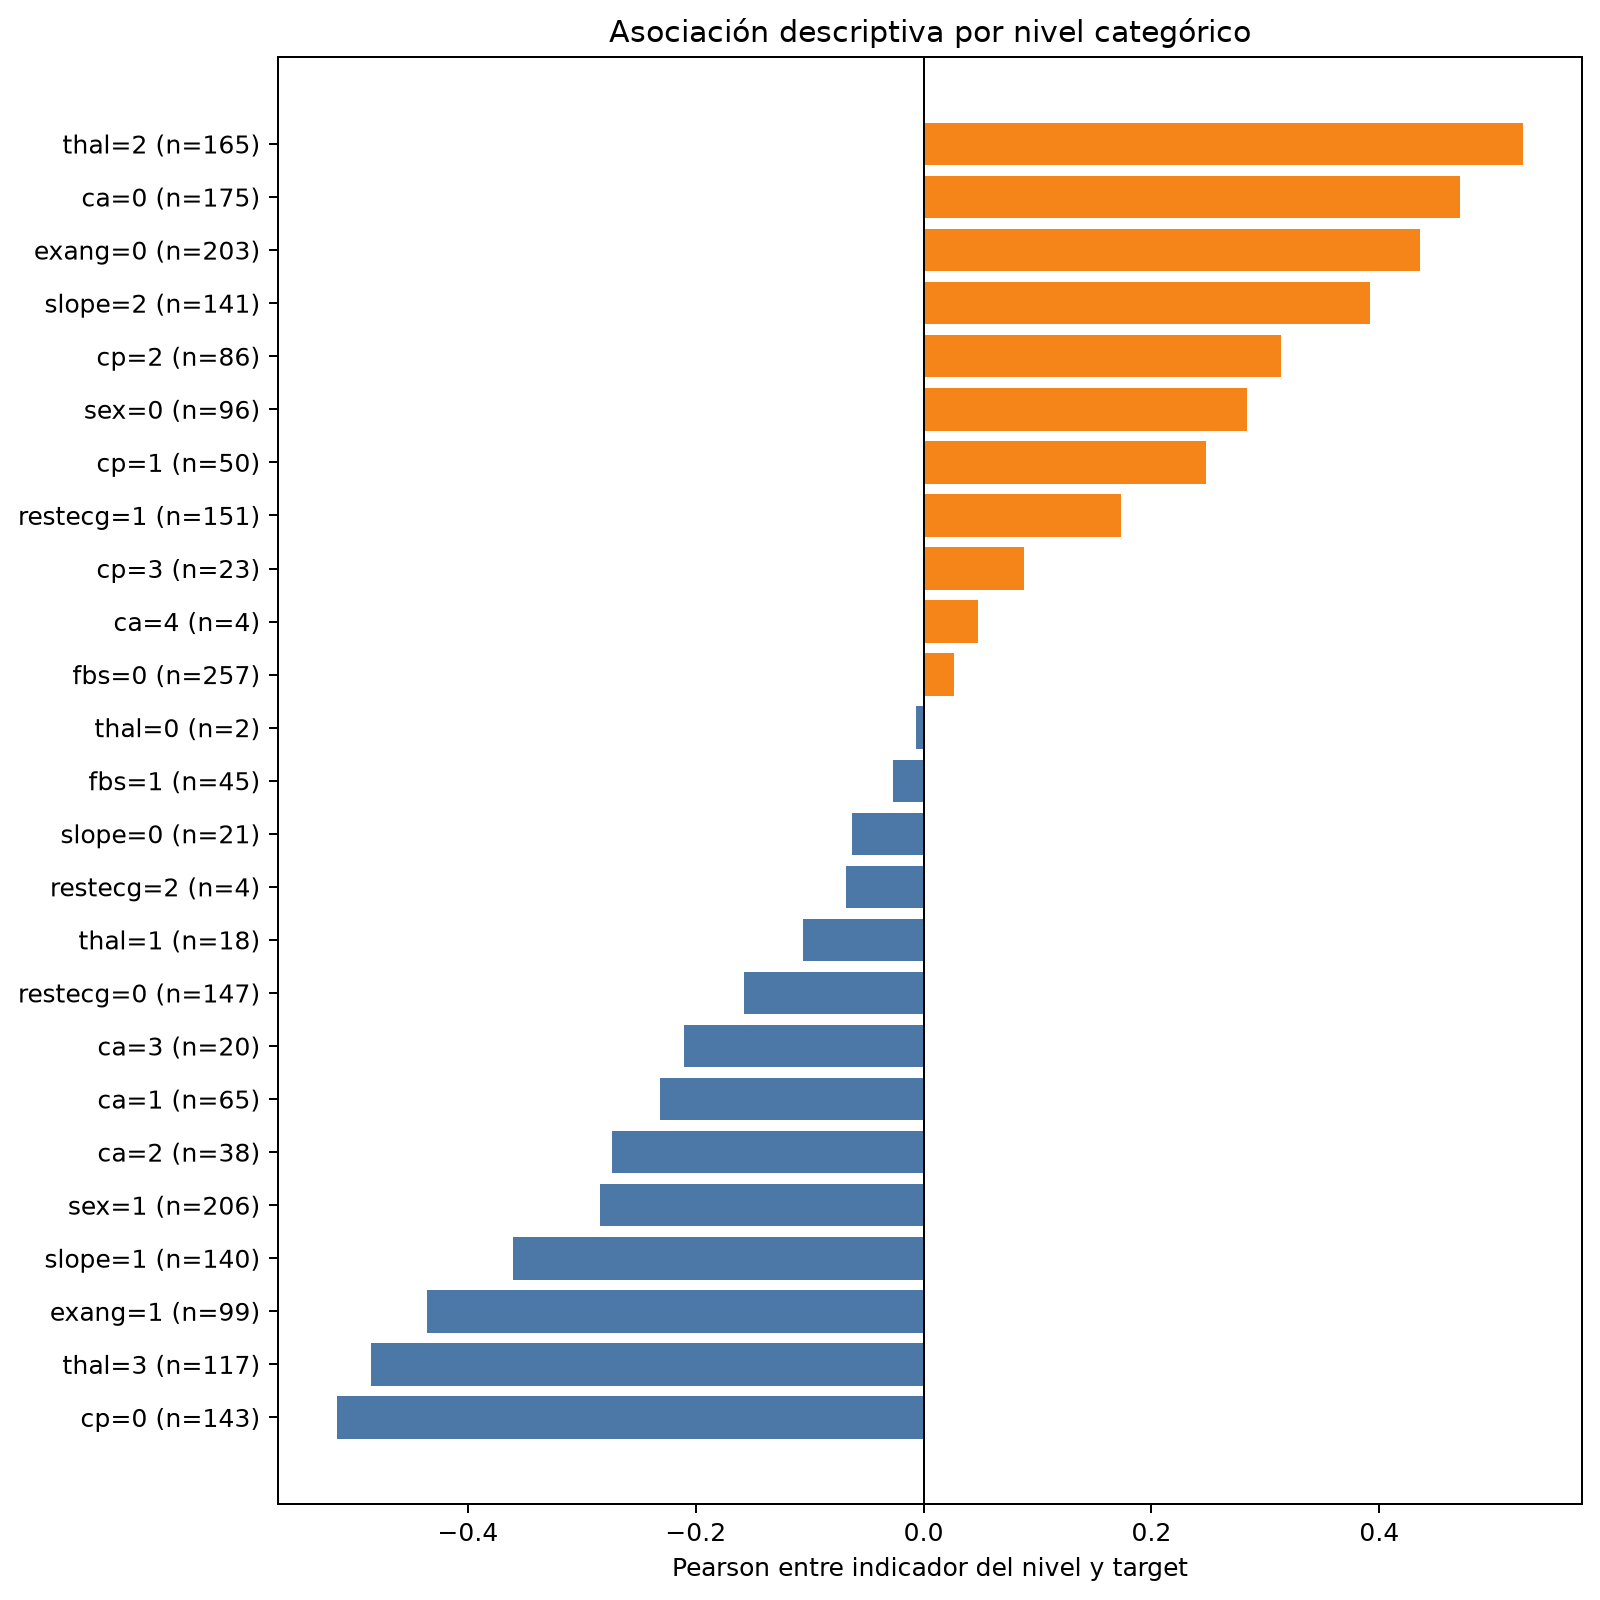
\includegraphics[width=0.91\textwidth]{../outputs/figures/asociacion_niveles_categoricos_target.png}
  \caption{Asociación descriptiva entre niveles categóricos y \texttt{target}; el tamaño muestral varía por nivel.}
  \label{fig:corr-cat}
\end{figure}

\section{Diseño experimental}
\subsection{Partición y validación}
Tras deduplicar, se separa 75\% para entrenamiento y 25\% para prueba mediante partición estratificada con semilla 42: 226 registros de entrenamiento y 76 de prueba. En entrenamiento se comparan candidatos con validación cruzada estratificada de cinco folds, aleatorizada con la misma semilla. Se ensayan dos transformaciones experimentales, sin usarlas para seleccionar el artefacto final: interacción $\texttt{oldpeak}\times\texttt{exang}$ en XGBoost y splines cuadráticas de tres nudos en regresión logística. La selección permanece restringida a candidatos XGBoost one-hot regulares que entrenan con CUDA. El conjunto de prueba retenido se usa para la comparación final reportada.

\subsection{Candidatos y configuración}
Se evaluaron una regresión logística de referencia (CPU, one-hot y RobustScaler), un XGBoost ordinal previo y dos XGBoost CUDA con variables categóricas one-hot. El XGBoost one-hot somero usa 250 estimadores, profundidad máxima 2, tasa de aprendizaje 0,04, \texttt{min\_child\_weight=3}, \texttt{subsample=0,9}, \texttt{colsample\_bytree=0,9} y regularización L2 de 2. El candidato one-hot regularizado usa 200 estimadores, profundidad 3, tasa 0,03, \texttt{min\_child\_weight=5}, subsampling y muestreo de columnas 0,85, L2 de 5. Ambos configuran objetivo binario logístico, métrica de entrenamiento logloss, método hist y dispositivo CUDA. La semilla es 42.

El artefacto final es el XGBoost one-hot somero, entrenado localmente con CUDA en la NVIDIA GeForce RTX 4060 Laptop GPU. Se eligió entre los candidatos GPU one-hot por ROC-AUC promedio de validación cruzada; la regresión logística obtuvo el promedio numérico más alto, pero es una referencia CPU y no el artefacto final seleccionado para este ejercicio.

\section{Resultados}
\begin{table}[H]
  \centering
  \caption{ROC-AUC medio (desviación estándar) en validación cruzada de entrenamiento}
  \label{tab:cv}
  \small
  \begin{tabularx}{\textwidth}{Xlr}
    \toprule
    Candidato & Dispositivo & ROC-AUC CV \\
    \midrule
    Regresión logística (one-hot + RobustScaler) & CPU & 0,919 (0,052) \\
    XGBoost ordinal previo & CUDA & 0,917 (0,062) \\
    XGBoost one-hot somero, seleccionado & CUDA & 0,914 (0,055) \\
    XGBoost one-hot regularizado & CUDA & 0,913 (0,061) \\
    XGBoost experimental, interacción $\texttt{oldpeak}\times\texttt{exang}$ & CUDA & 0,912 (0,056) \\
    Logística experimental, splines + one-hot & CPU & 0,904 (0,043) \\
    \bottomrule
  \end{tabularx}
\end{table}

\begin{figure}[H]
  \centering
  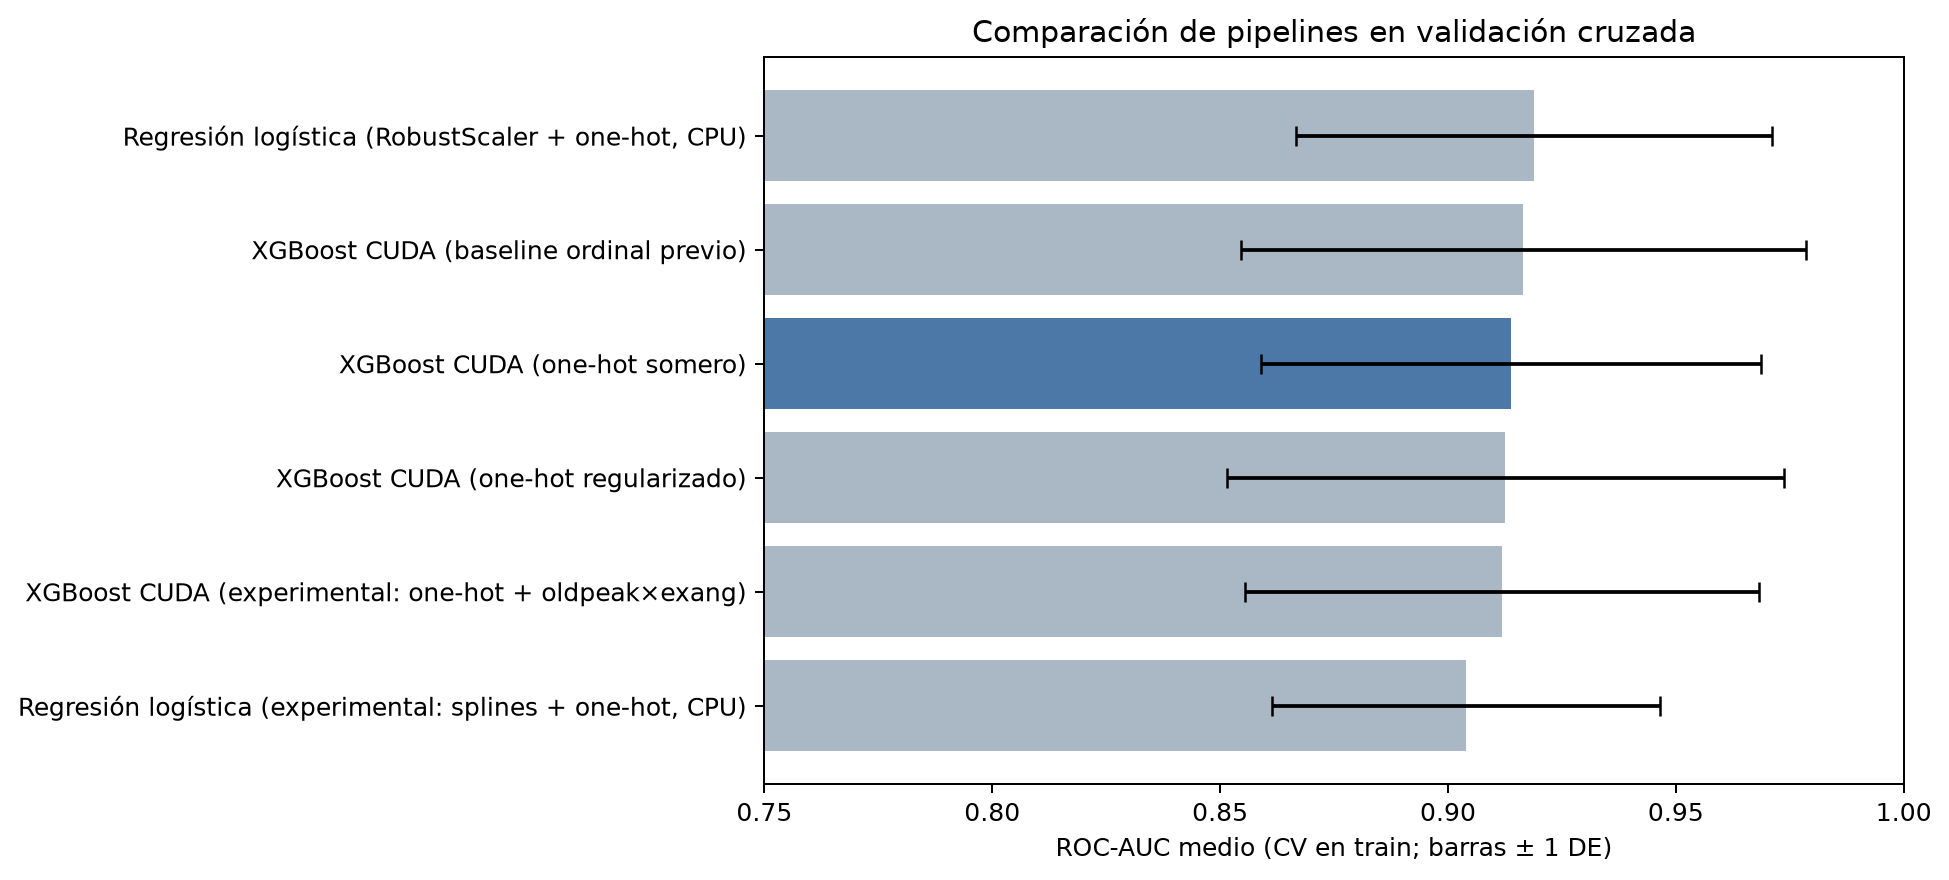
\includegraphics[width=0.91\textwidth]{../outputs/figures/comparacion_roc_auc_validacion_cruzada.png}
  \caption{Comparación del ROC-AUC medio y su dispersión entre folds. La variabilidad es apreciable dada la muestra pequeña.}
  \label{fig:cv}
\end{figure}

En la comprobación con diez repeticiones de cinco folds, la interacción XGBoost promedió ROC-AUC 0,91279 frente a 0,91262 de su referencia (delta $+0,00016$); el cambio favoreció al candidato en cuatro repeticiones y a la referencia en seis (mediana $-0,00078$). La logística con splines promedió 0,90099 frente a 0,91897 y fue inferior en las diez repeticiones (delta medio $-0,01798$). La señal de la interacción es prácticamente nula y no consistente; la de splines es negativa en estos folds. Las repeticiones comparten observaciones, así que no constituyen 50 muestras independientes ni una prueba de significación. Ninguna transformación se incorpora al artefacto final.

\paragraph{Justificación de la decisión.} No se implementa la interacción explícita porque no ofrece una ganancia reproducible que compense añadir otra transformación: el XGBoost de profundidad 2 ya puede aprender interacciones simples mediante divisiones sucesivas, y el delta observado se centra prácticamente en cero. Tampoco se implementan splines: aumentan los grados de libertad de la referencia logística con sólo 226 registros de entrenamiento y su ROC-AUC fue menor en las diez repeticiones. Mantenerlas sin evidencia de mejora agregaría complejidad y riesgo de ajustar particularidades de esta muestra. La conclusión se limita a estos candidatos y datos; no afirma que cualquier ingeniería de variables sea inútil.

\begin{figure}[H]
  \centering
  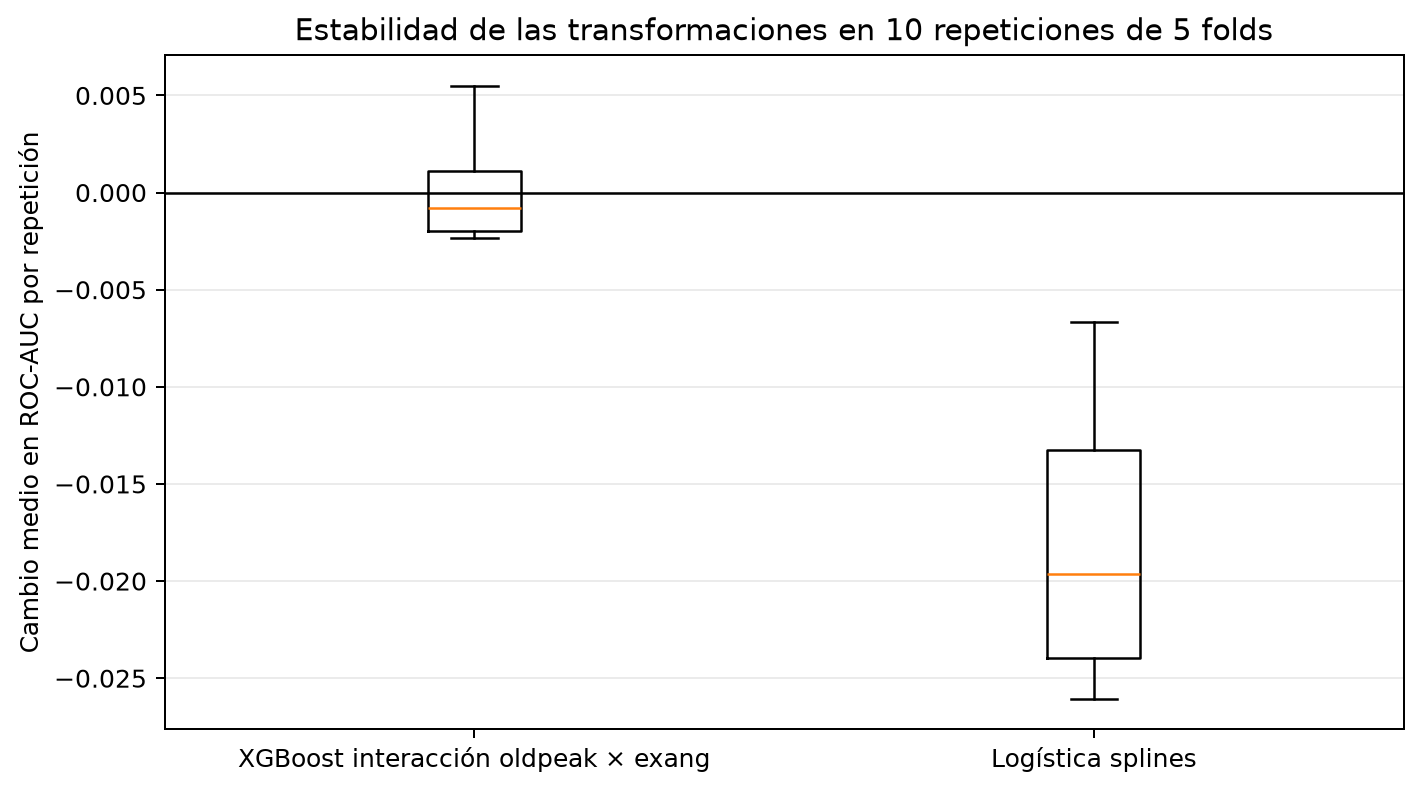
\includegraphics[width=0.78\textwidth]{../outputs/figures/feature_engineering_repeated_cv.png}
  \caption{Diferencias medias de ROC-AUC por repetición de cinco folds para cada transformación frente a su referencia.}
  \label{fig:feature-engineering-cv}
\end{figure}

En los 76 registros de prueba, el XGBoost one-hot seleccionado obtuvo accuracy 0,776, precisión de clase 1 de 0,786, recall 0,805, F1 0,795 y ROC-AUC 0,875. El baseline ordinal previo obtuvo 0,789, 0,791, 0,829, 0,810 y 0,875, respectivamente. Las matrices de confusión muestran 60 aciertos del baseline y 59 del one-hot. Ambos tuvieron 26 verdaderos negativos y 9 falsos positivos; el baseline tuvo 34 verdaderos positivos y 7 falsos negativos, frente a 33 y 8 del one-hot. Por tanto, la ventaja de accuracy es 1/76, equivalente a 1,32 puntos porcentuales, explicada por un solo caso positivo adicional acertado. No es evidencia de una superioridad estable del pipeline ordinal. Las curvas ROC empatan en AUC=0,875: la discriminación agregada es la misma en esta prueba, aunque el conteo al umbral predeterminado cambia por un caso. La codificación one-hot sigue siendo la decisión más coherente para categorías nominales, pues no impone un orden artificial entre códigos. Este resultado pequeño no demuestra equivalencia ni diferencia estadística.

\begin{table}[H]
  \centering
  \caption{Métricas en el mismo conjunto de prueba retenido}
  \label{tab:test}
  \begin{tabular}{lrr}
    \toprule
    Métrica & XGBoost ordinal previo & XGBoost one-hot seleccionado \\
    \midrule
    Accuracy & 0,789 & 0,776 \\
    Precisión (clase 1) & 0,791 & 0,786 \\
    Recall (clase 1) & 0,829 & 0,805 \\
    F1 (clase 1) & 0,810 & 0,795 \\
    ROC-AUC & 0,875 & 0,875 \\
    \bottomrule
  \end{tabular}
\end{table}

\begin{figure}[H]
  \centering
  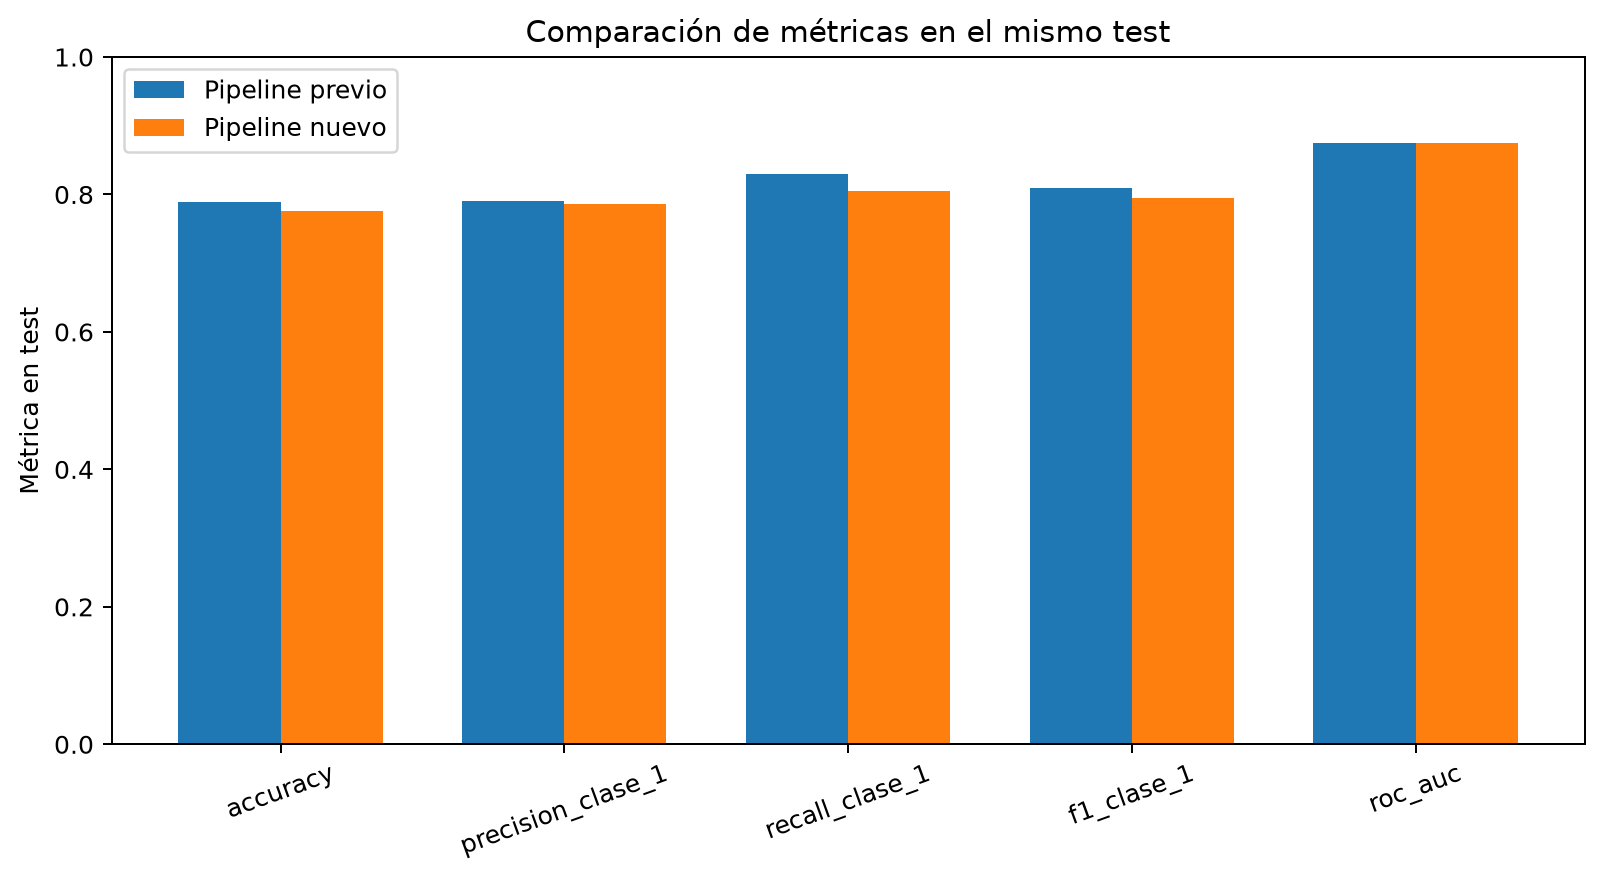
\includegraphics[width=0.91\textwidth]{../outputs/figures/comparacion_metricas_test_antes_despues.png}
  \caption{Métricas de ambos pipelines sobre la misma partición retenida.}
  \label{fig:test}
\end{figure}

\begin{figure}[H]
  \centering
  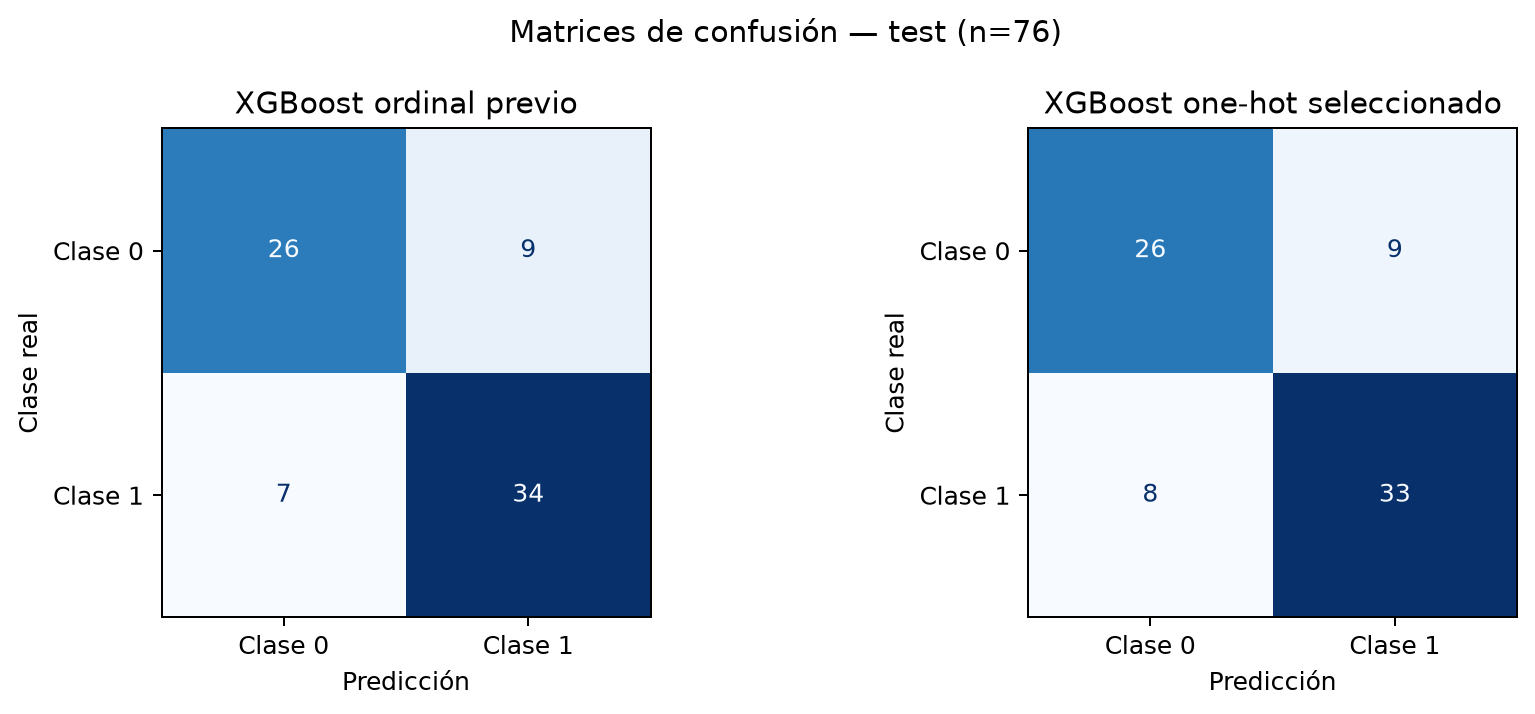
\includegraphics[width=0.92\textwidth]{../outputs/figures/matrices_confusion_test_comparacion.png}
  \caption{Matrices de confusión sobre la prueba retenida. La ventaja de accuracy del baseline es un único caso positivo adicional correctamente clasificado.}
  \label{fig:matrices-test}
\end{figure}

\begin{figure}[H]
  \centering
  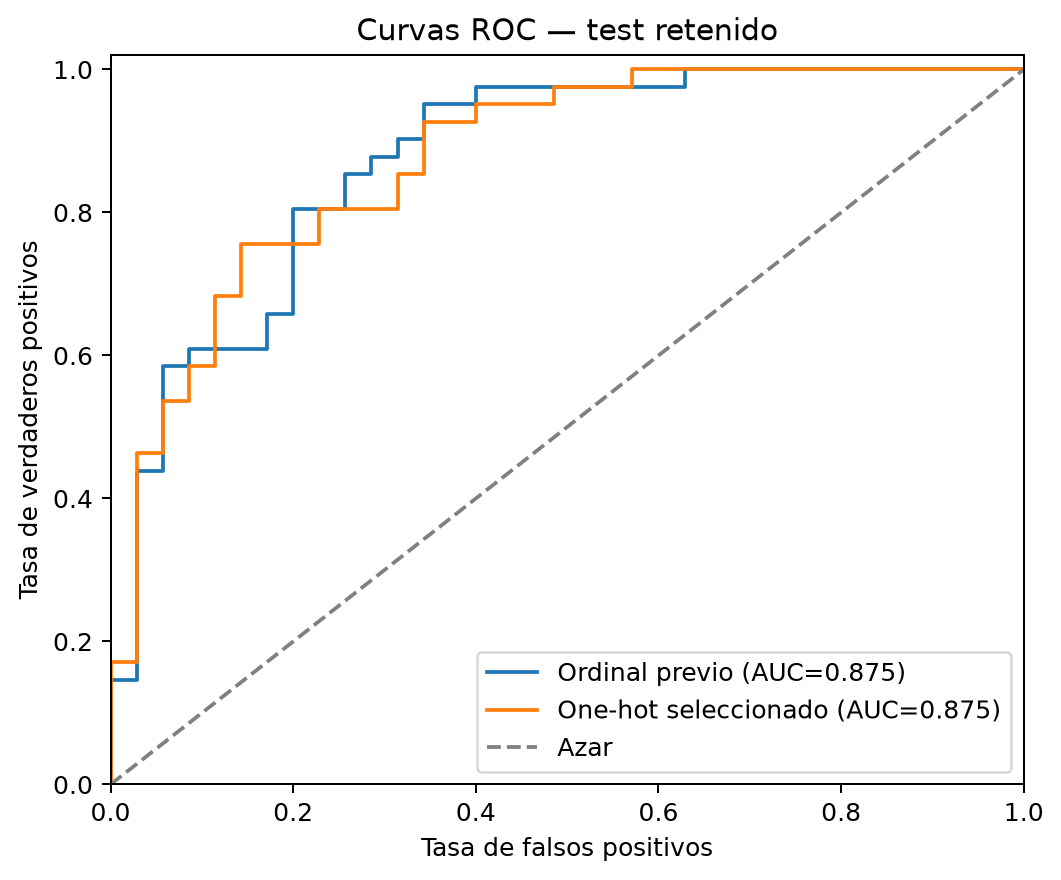
\includegraphics[width=0.76\textwidth]{../outputs/figures/curvas_roc_test_comparacion.png}
  \caption{Curvas ROC de los dos pipelines en test; ambos obtienen AUC=0,875.}
  \label{fig:roc-test}
\end{figure}

\subsection{Explicabilidad global y local}
La matriz de confusión muestra conteos de aciertos y errores; no atribuye su origen a los predictores. Se extrajeron contribuciones TreeSHAP nativas de XGBoost con \texttt{pred\_contribs}. En el pipeline one-hot, las contribuciones de sus indicadores se agruparon por variable fuente; en el baseline ordinal se explicaron las 13 columnas tal como fueron entregadas al árbol. En ambos casos, la suma de contribuciones más el valor base reconstruye el margen log-odds, verificado numéricamente. Esta descomposición explica la salida del modelo, no causalidad \parencite{xgboost-pred-contribs}.

Ambos modelos destacan las mismas tres variables en el promedio absoluto sobre los 302 registros únicos: \texttt{cp} (one-hot 0,971; ordinal 0,872), \texttt{ca} (0,855; 0,643) y \texttt{thal} (0,599; 0,479), en unidades de margen log-odds. Después aparecen \texttt{oldpeak} (0,407; 0,362), \texttt{sex} (0,395; 0,248) y \texttt{thalach} (0,346; 0,210). Ambos asignaron contribución cero a \texttt{fbs} en los registros explicados; esto describe estos artefactos, no la relevancia clínica de la variable. La dirección de los valores positivos/negativos se refiere a empujar el score hacia las clases codificadas 1/0, cuya equivalencia clínica no está confirmada. El baseline ordinal recibe categorías como enteros y puede imponer umbrales dependientes del orden numérico; sus atribuciones deben interpretarse con esta salvedad.

\begin{figure}[H]
  \centering
  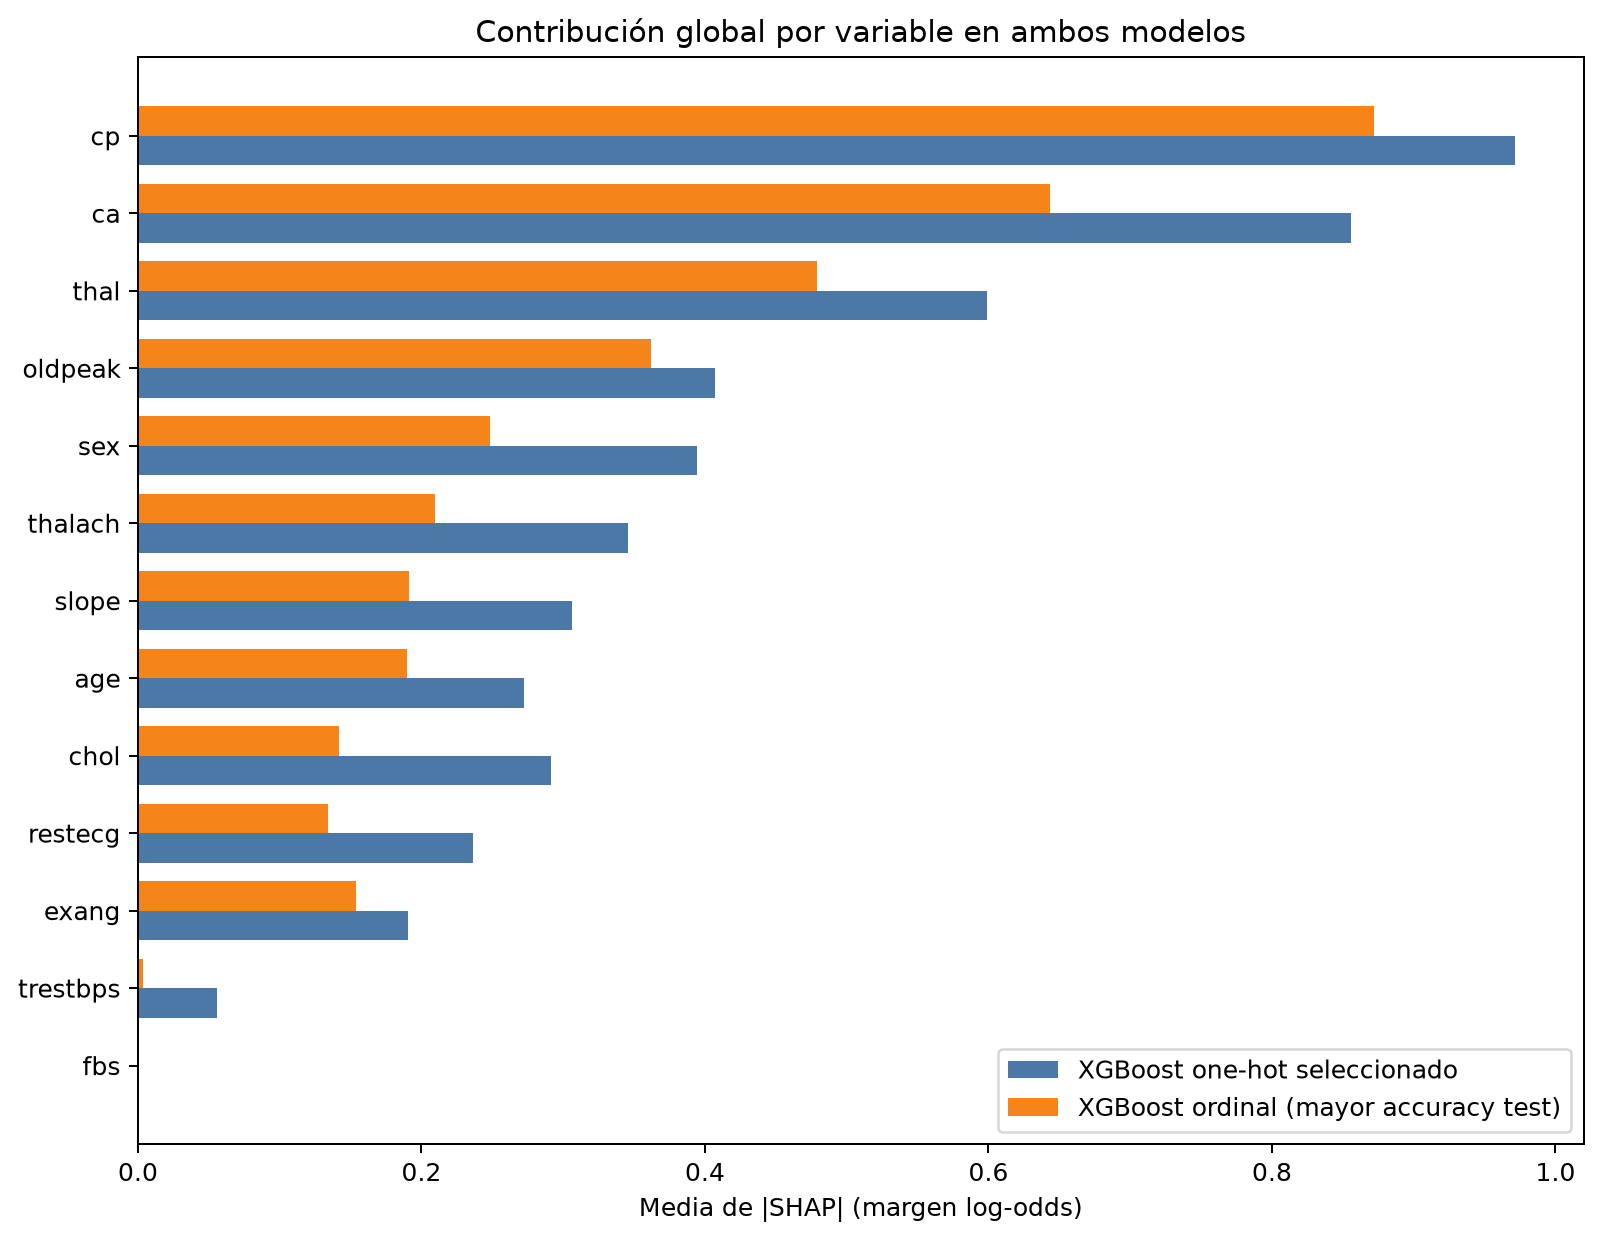
\includegraphics[width=0.90\textwidth]{../outputs/figures/shap_importancia_comparacion.png}
  \caption{Media global de contribuciones SHAP absolutas por variable original para el XGBoost one-hot y el baseline ordinal.}
  \label{fig:shap-global-modelo}
\end{figure}

\begin{figure}[H]
  \centering
  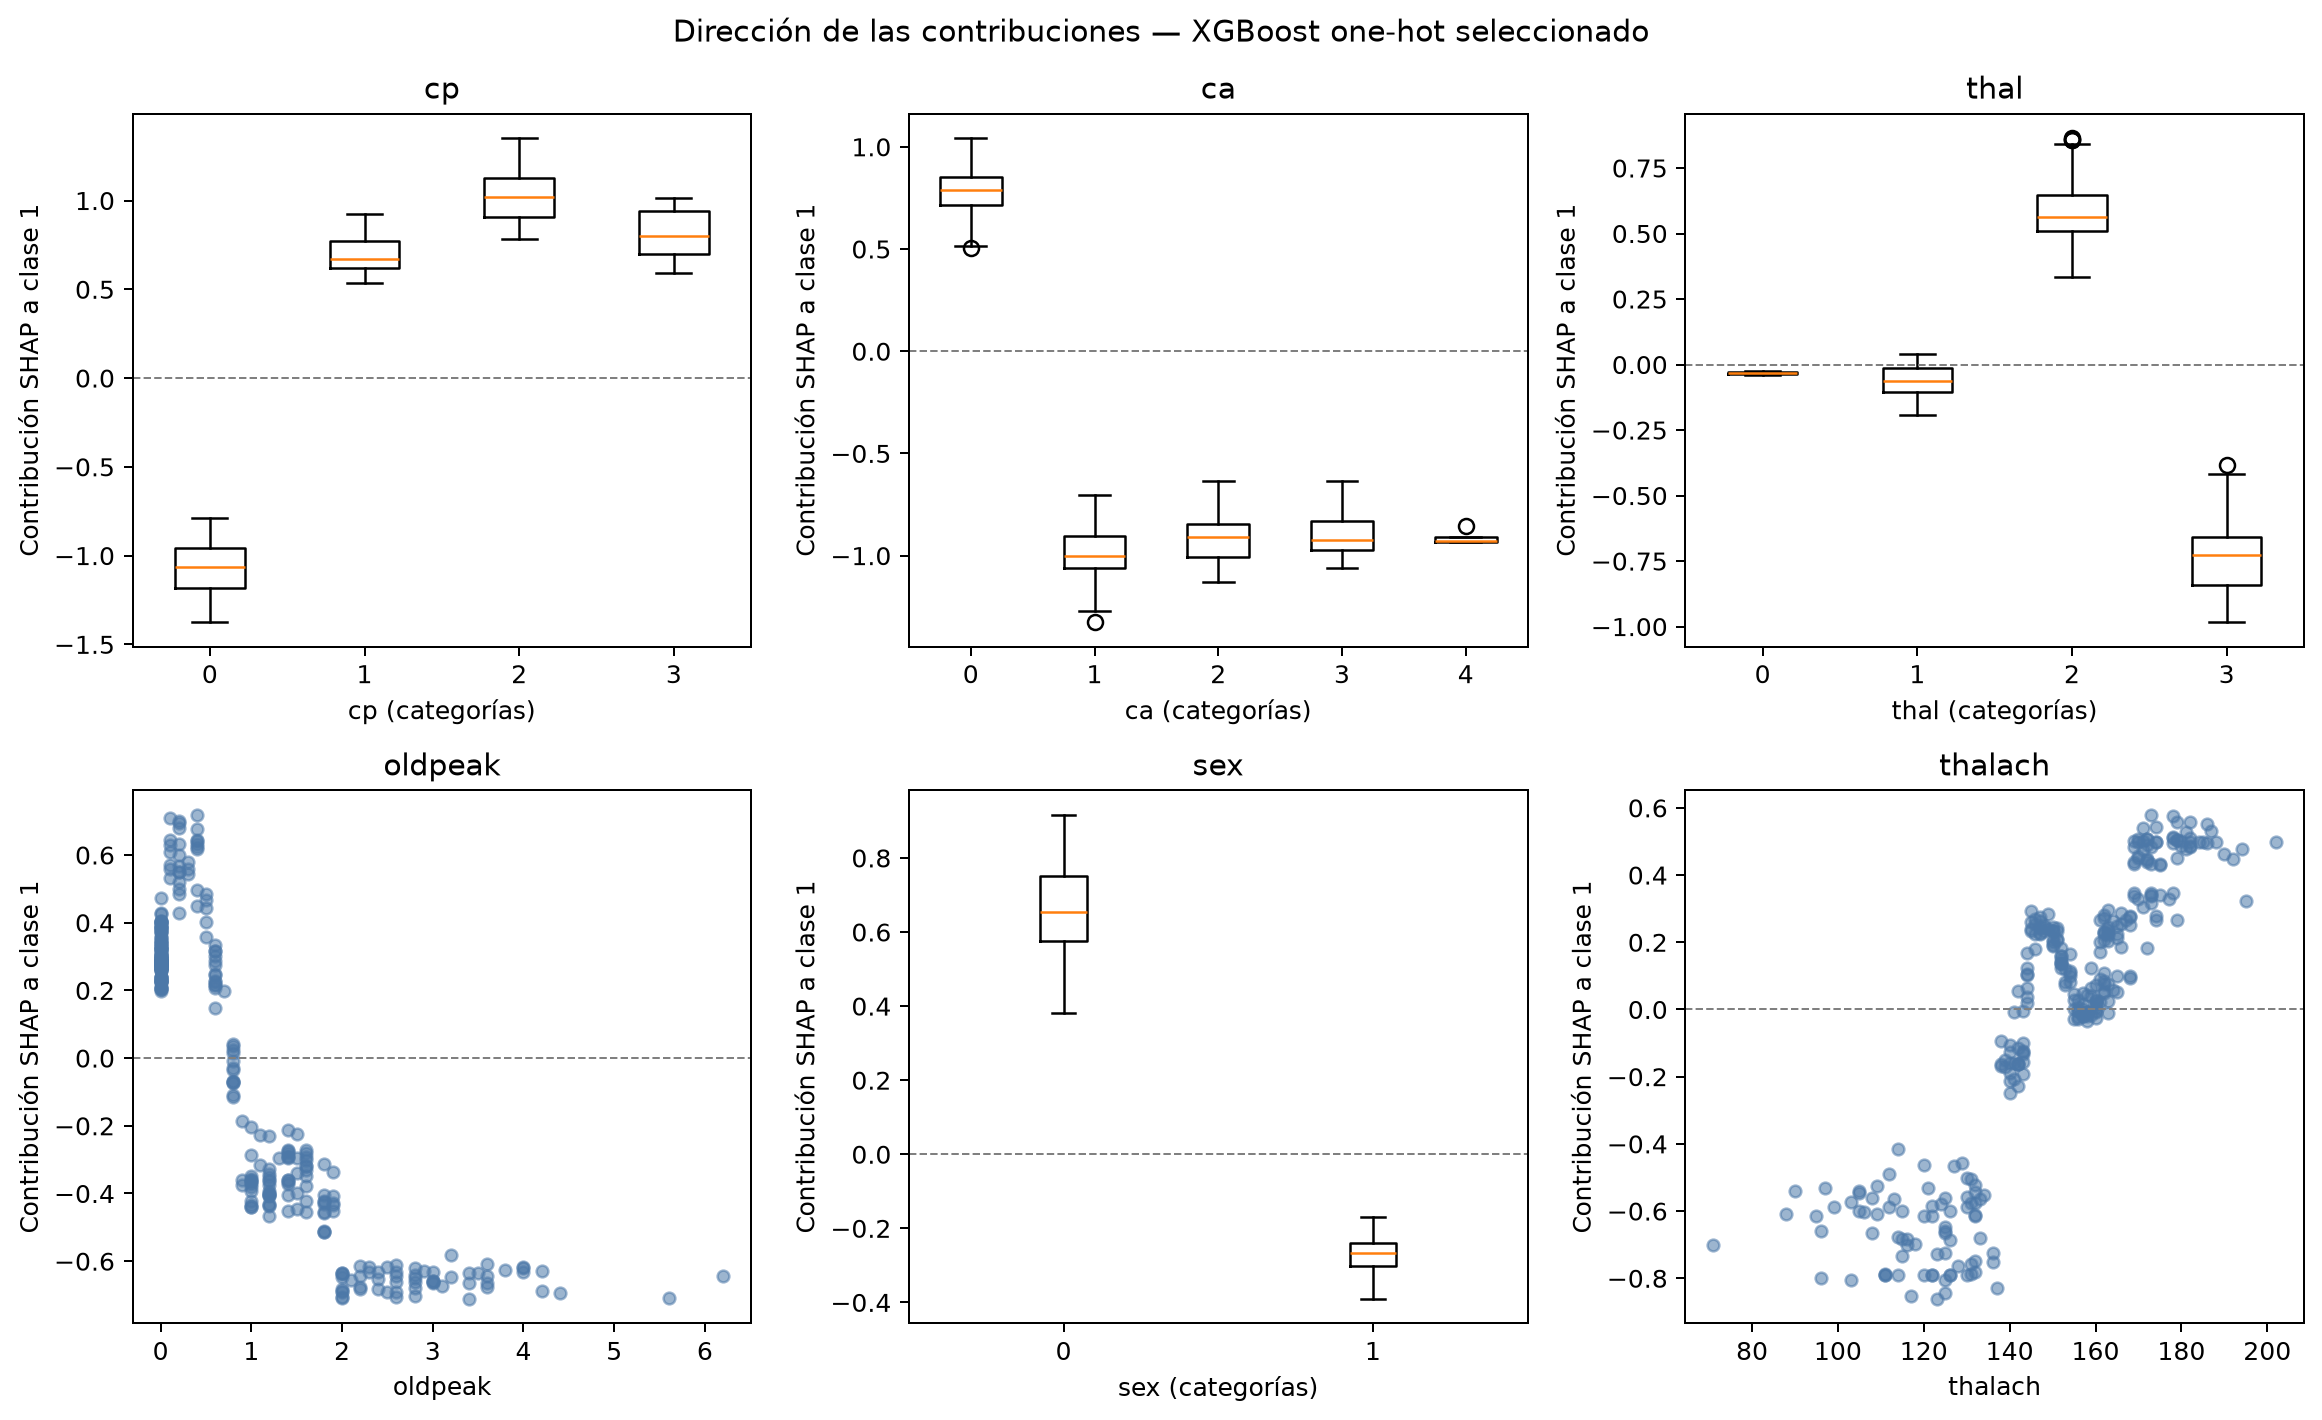
\includegraphics[width=0.98\textwidth]{../outputs/figures/shap_relacion_valor_atribucion.png}
  \caption{Atribuciones del pipeline one-hot según valor cuantitativo o nivel categórico. Cada nivel categórico aparece separado; el eje no define un orden entre códigos.}
  \label{fig:shap-direccion-modelo}
\end{figure}

Para explicar el modelo con mayor accuracy (baseline ordinal, 60/76) se descompusieron un falso negativo (fila 5: real 1, predicho 0, score de clase 1 0,388) y un falso positivo (fila 33: real 0, predicho 1, score 0,852). Como contraste, el pipeline one-hot (59/76) produjo en esas filas scores 0,300 y 0,848. Los números de fila son índices técnicos, no identificadores de personas. Las atribuciones indican qué variables empujaron los scores calculados, no por qué ocurrió el resultado real.

\begin{figure}[H]
  \centering
  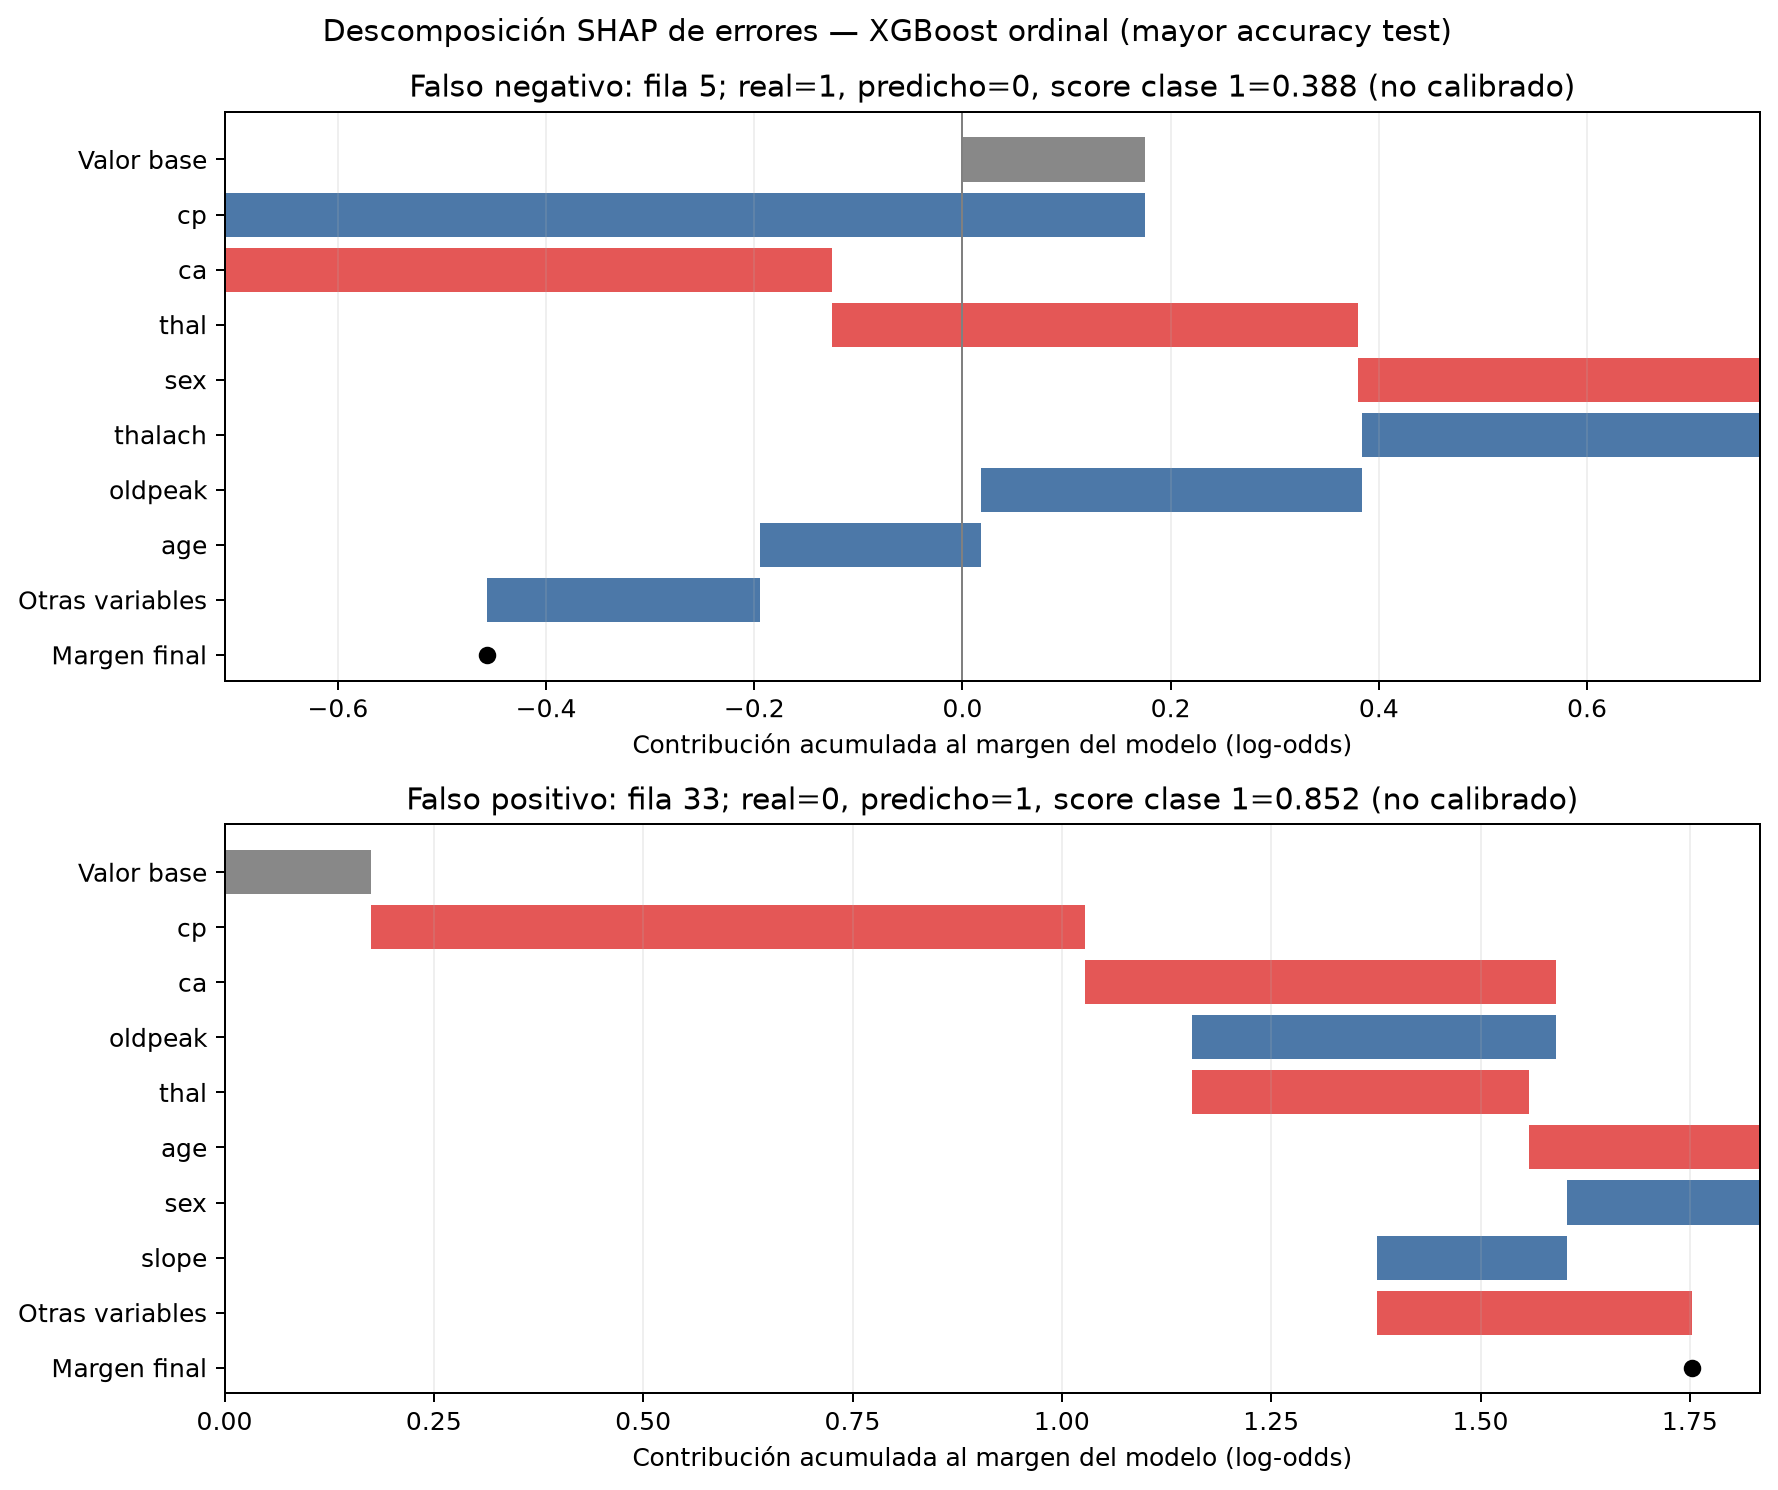
\includegraphics[width=0.98\textwidth]{../outputs/figures/shap_explicacion_casos_error_ordinal.png}
  \caption{Atribuciones por variable en dos errores del baseline ordinal, que tuvo el mayor accuracy en test. Rojo empuja hacia clase 1; azul hacia clase 0. Scores no calibrados.}
  \label{fig:shap-local-modelo}
\end{figure}

\begin{figure}[H]
  \centering
  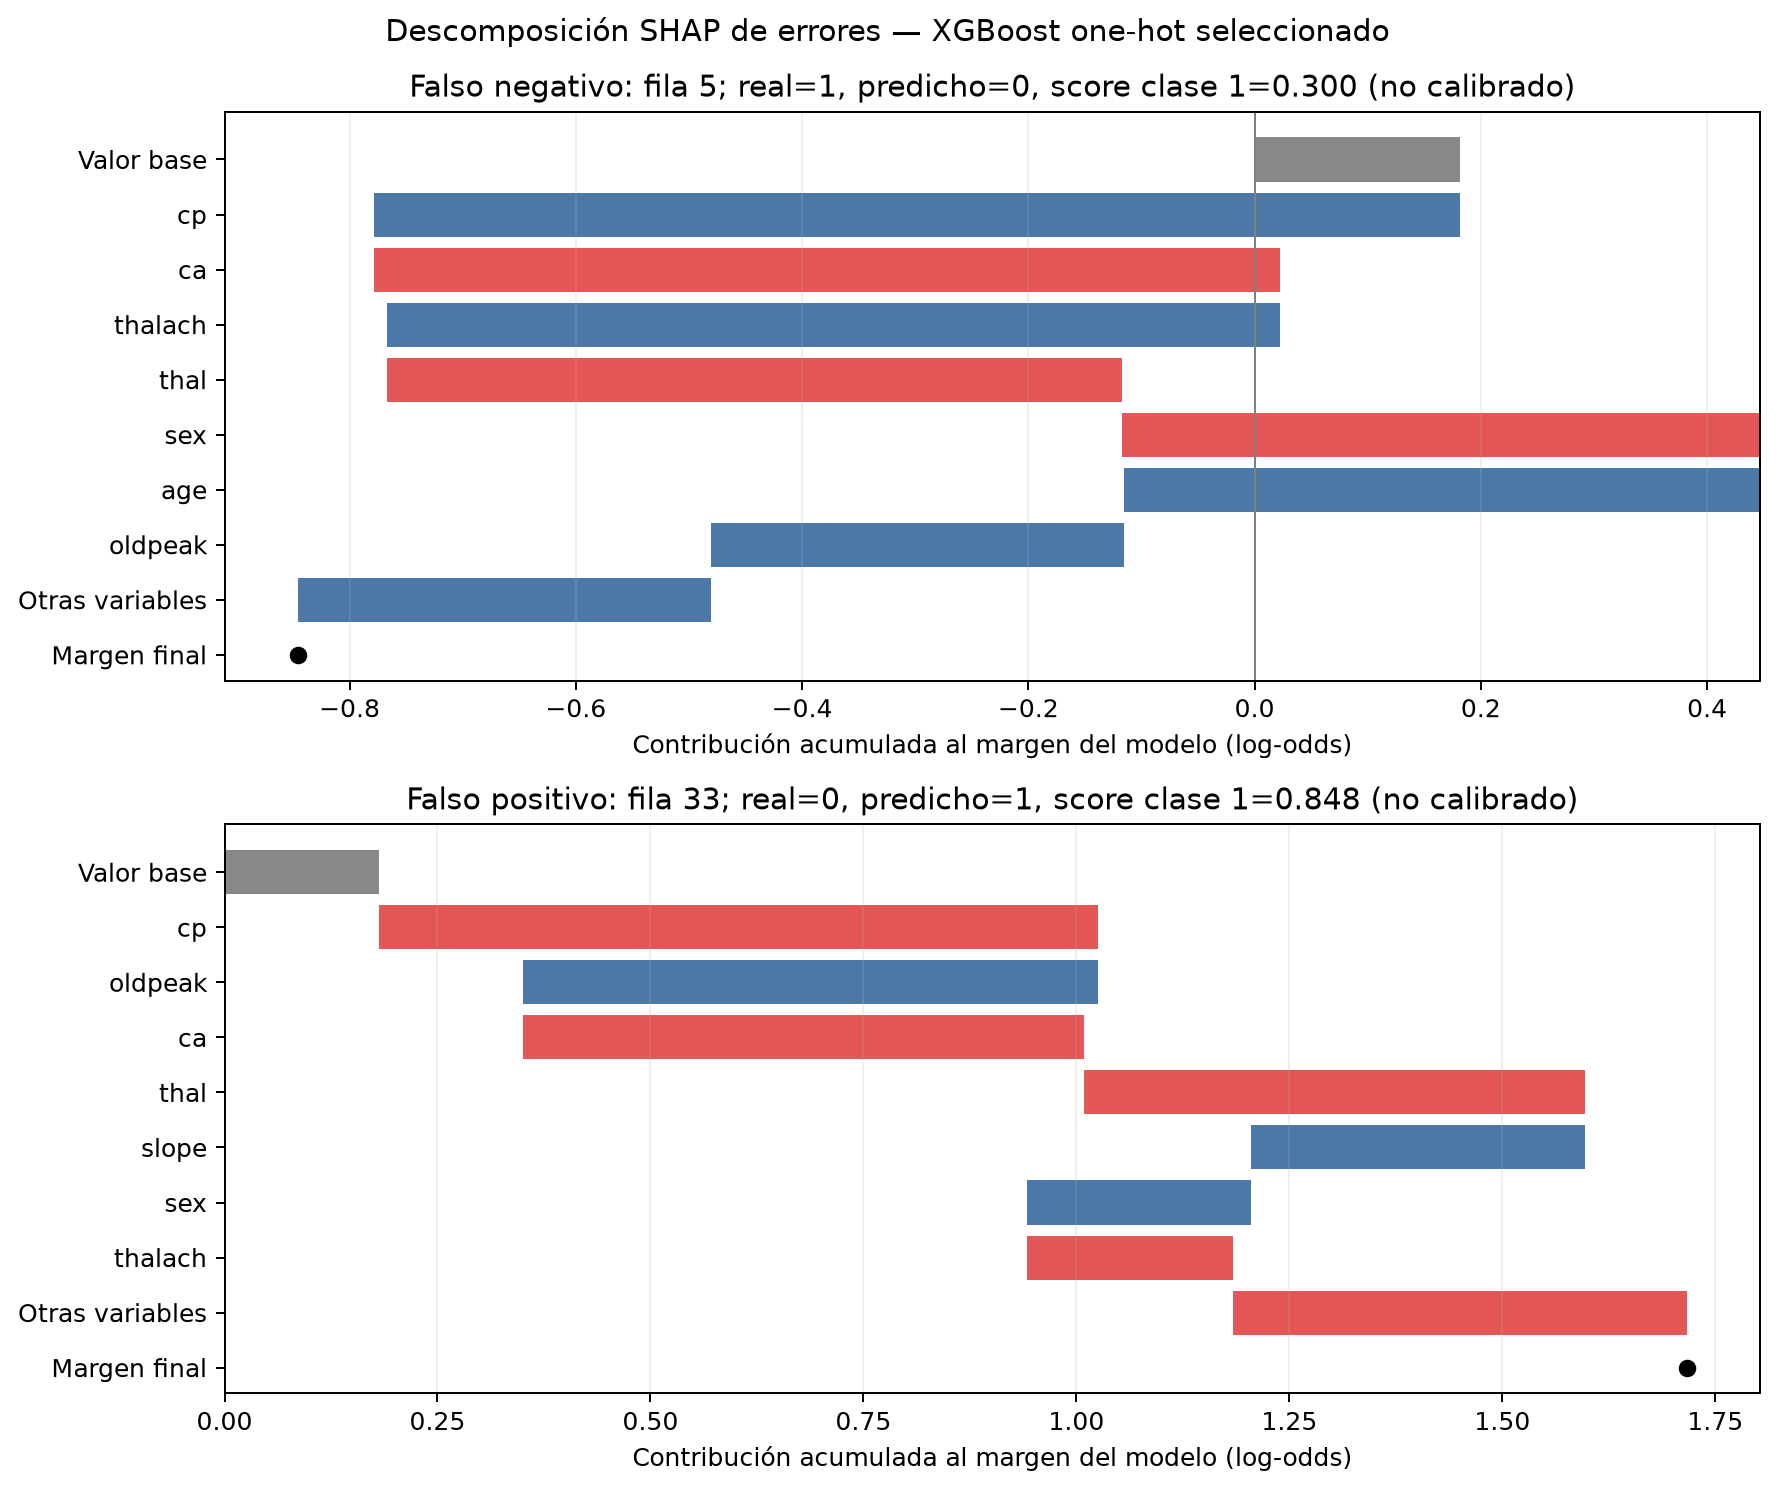
\includegraphics[width=0.98\textwidth]{../outputs/figures/shap_explicacion_casos_error.png}
  \caption{Mismos dos registros explicados con el XGBoost one-hot seleccionado.}
  \label{fig:shap-local-onehot}
\end{figure}

Las magnitudes SHAP dependen del modelo y de la muestra explicada: resumen cómo cada artefacto distribuye sus márgenes, no causalidad, importancia clínica ni equidad. El resumen global usa los 302 registros observados; la prueba de 76 se conserva para las métricas predictivas y los ejemplos locales.

\subsection{Todos los errores y análisis por subgrupo}
Se extendió la explicación local a los 17 errores del test one-hot (8 falsos negativos y 9 falsos positivos), sin volver a entrenar ni cambiar los 76 casos de prueba. Entre ambos tipos de error, \texttt{cp}, \texttt{ca} y \texttt{thal} tienen las mayores contribuciones absolutas medias. Para los falsos negativos, la contribución firmada media de \texttt{cp} fue $-0,565$ y la de \texttt{thalach} $-0,514$ log-odds; para los falsos positivos, \texttt{cp} fue $+0,558$ y \texttt{ca} $+0,566$. SHAP indica la dirección del score calculado en estos registros, no la causa del desenlace.

\begin{figure}[H]
  \centering
  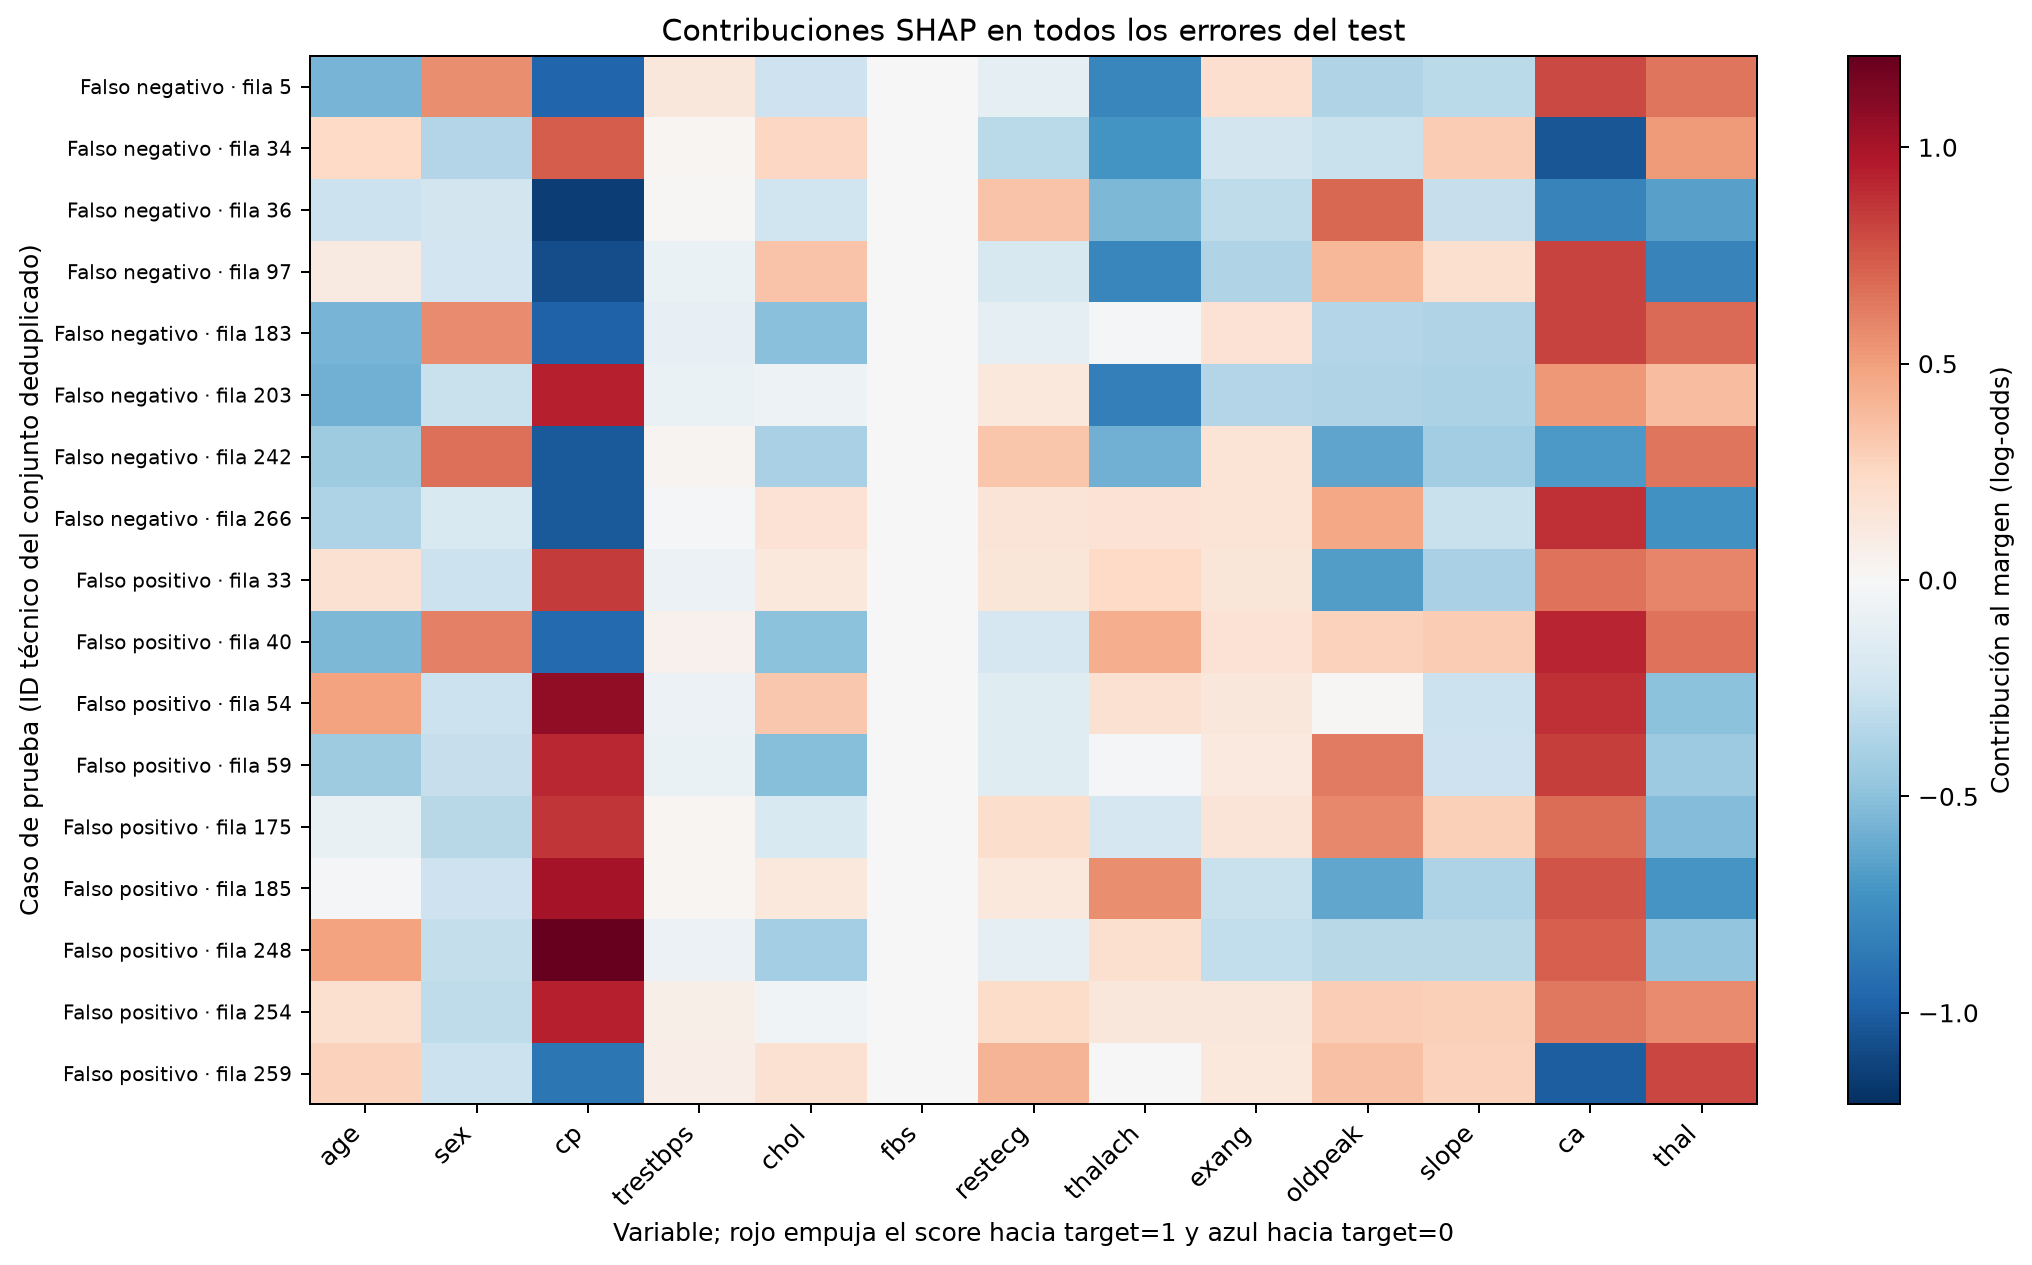
\includegraphics[width=0.98\textwidth]{../outputs/figures/shap_mapa_errores_test.png}
  \caption{Contribuciones SHAP de todas las variables en cada error del test. Cada fila es un caso; los IDs son índices técnicos del conjunto deduplicado.}
  \label{fig:shap-mapa-errores}
\end{figure}

\begin{figure}[H]
  \centering
  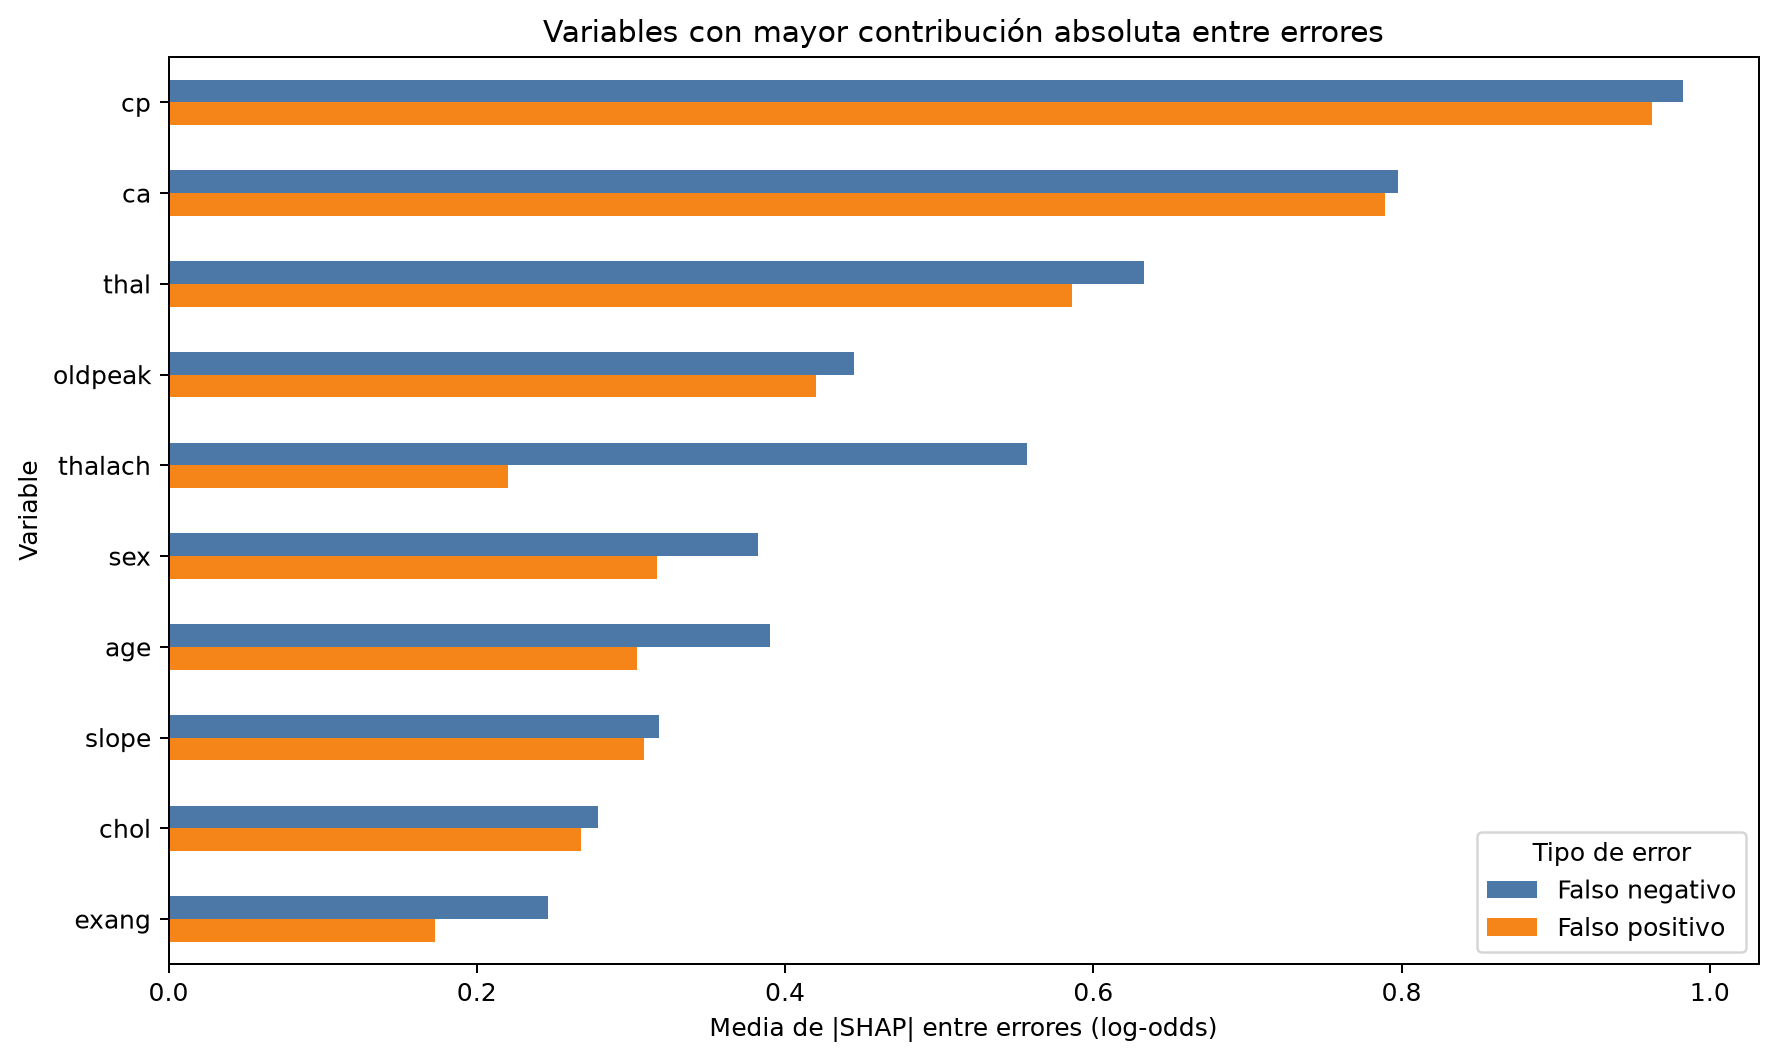
\includegraphics[width=0.9\textwidth]{../outputs/figures/shap_resumen_errores_test.png}
  \caption{Media de contribución absoluta para las variables más influyentes entre falsos positivos y negativos (9 y 8 casos).}
  \label{fig:shap-resumen-errores}
\end{figure}

En la prueba, el código \texttt{sex=0} reúne 22 casos (recall $0,813$, especificidad $0,833$) y \texttt{sex=1}, 54 (recall $0,800$, especificidad $0,724$). Los intervalos Wilson del 95\% son amplios y se solapan. En los grupos etarios de 60--69 años (n=25), recall fue $0,500$ y especificidad $0,824$; en 50--59 (n=29), $0,778$ y $0,727$. Los grupos menores de 40 y de 70 o más tienen sólo tres casos cada uno y no permiten inferencias. La bandera de soporte bajo se activa si el grupo tiene menos de 10 filas o menos de cinco casos en cualquiera de las clases.

\begin{figure}[H]
  \centering
  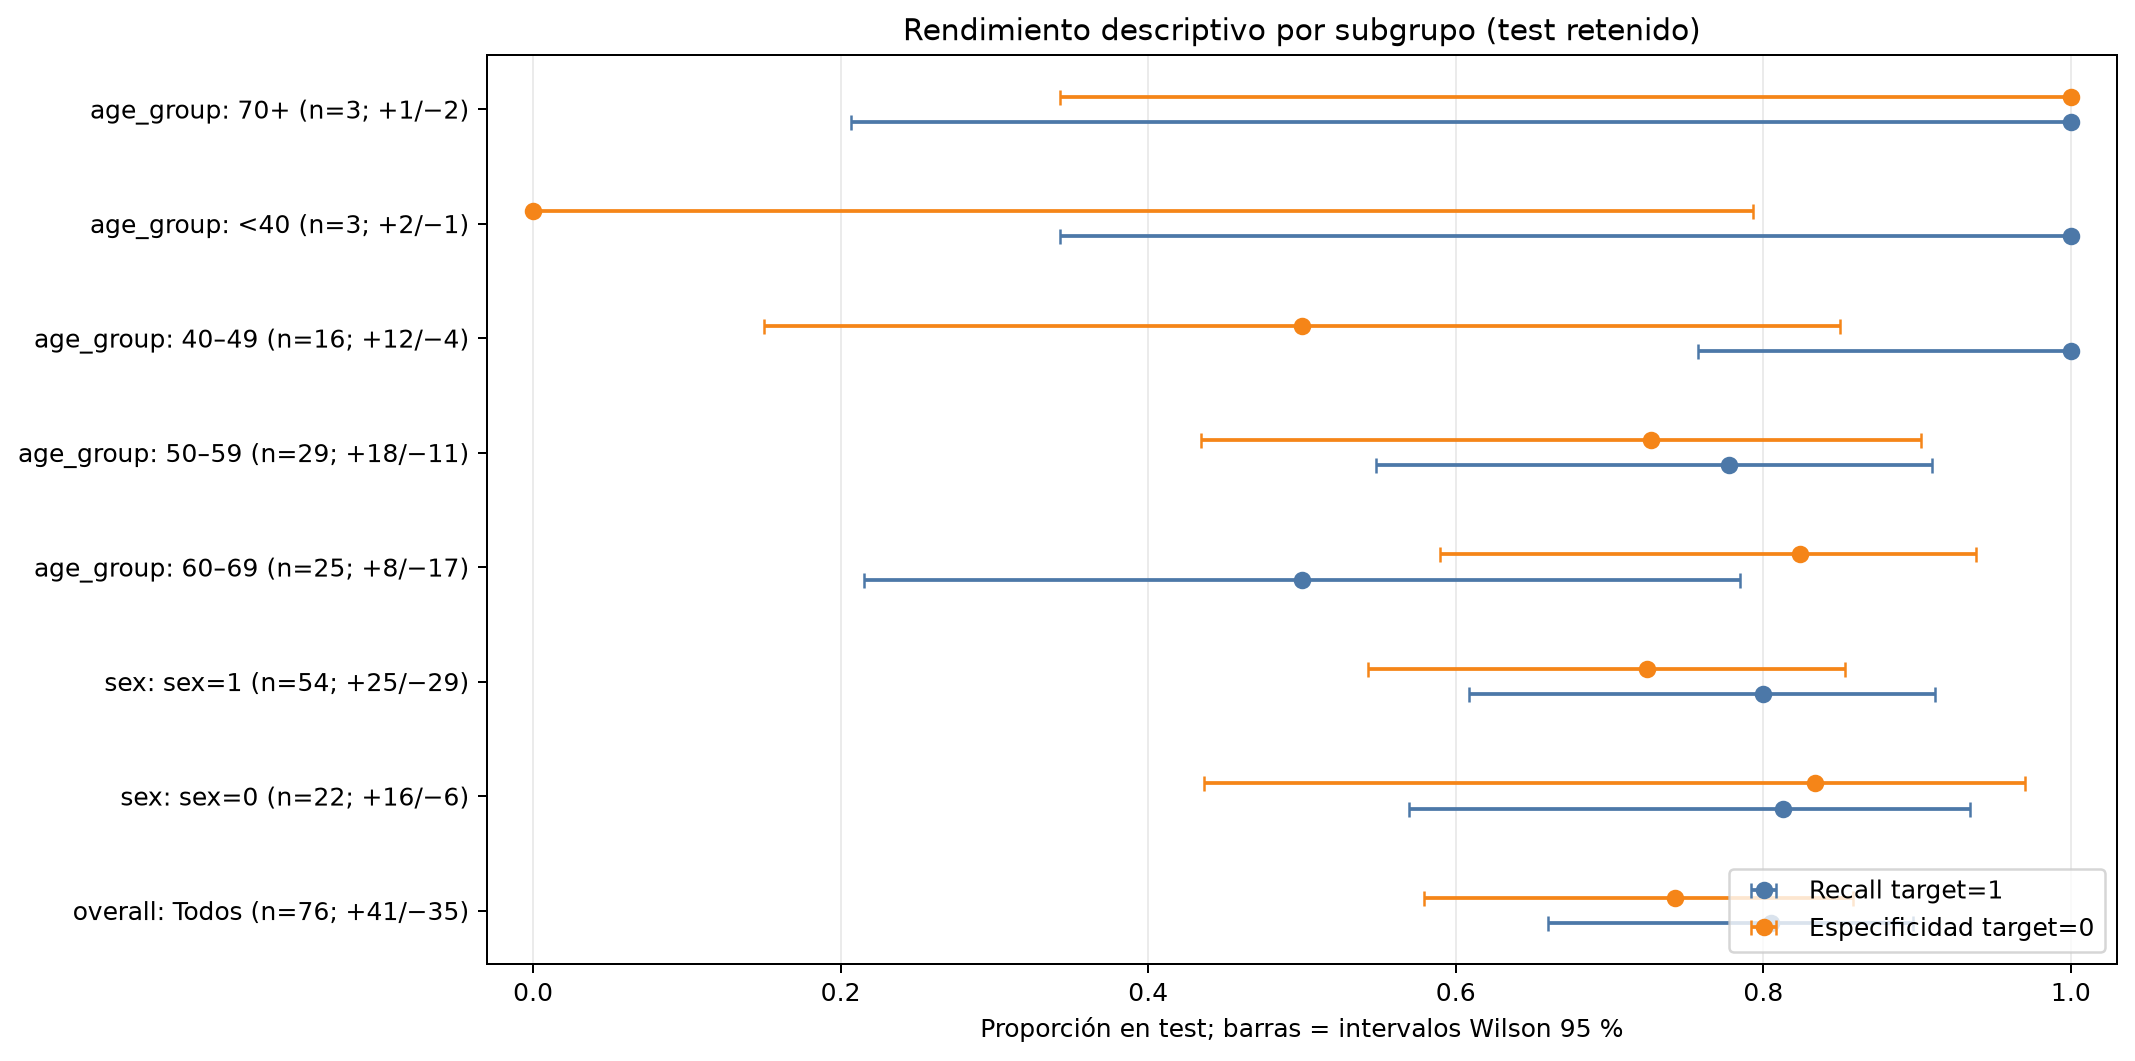
\includegraphics[width=0.95\textwidth]{../outputs/figures/metricas_test_por_subgrupo.png}
  \caption{Recall y especificidad por códigos de sexo y rangos etarios, con tamaños y conteos de clase en las etiquetas e intervalos Wilson del 95\%. Los grupos pequeños no sustentan comparaciones concluyentes.}
  \label{fig:metricas-subgrupos}
\end{figure}

El dataset deduplicado tiene 138 etiquetas 0 y 164 etiquetas 1, sin un desbalance global fuerte. La distinta representación por código de sexo y los tamaños reducidos siguen siendo riesgos de cobertura. Estas métricas de una sola partición no prueban ni descartan sesgo; no se realiza una afirmación de equidad. El análisis es reproducible con el notebook 06 de auditoría de errores y subgrupos; sus tablas están en \texttt{outputs/tables/}.

\section{Evaluación anidada, calibración y umbrales}
Como análisis complementario se ejecutó validación cruzada estratificada anidada, con tres repeticiones de cinco folds externos y tres folds internos. En cada fold externo, la familia y los hiperparámetros se seleccionaron por ROC-AUC interno. La calibración sigmoide y la selección de umbrales se ajustaron dentro del entrenamiento externo; el fold externo sólo se utilizó para evaluar. Este diseño reduce el optimismo al separar selección y evaluación, aunque las tres repeticiones comparten registros y no son muestras independientes.

El ROC-AUC externo fue 0,9112 (desviación 0,0104 entre las tres medias por repetición), tanto antes como después de la calibración. Brier bajó de 0,1197 a 0,1169 y log-loss de 0,3914 a 0,3745, mejoras modestas en la muestra evaluada. Con umbral 0,5 calibrado, balanced accuracy fue 0,8366, recall de clase 1 fue 0,8739 y especificidad de clase 0 fue 0,7993. El umbral que optimizó balanced accuracy dentro del entrenamiento promedió 0,5330 y obtuvo 0,8319 en los folds externos; el umbral que optimizó F1 promedió 0,4163, alcanzó recall 0,8941 pero redujo especificidad a 0,7557 y balanced accuracy a 0,8249. Ningún umbral alternativo mejoró consistentemente el balance externo. No se recomienda un punto de operación clínica.

La regresión logística fue seleccionada en 14 de los 15 folds externos y XGBoost en uno. Esto justifica incluir logística en futuras evaluaciones si se permite CPU, pero no demuestra superioridad definitiva ni reemplaza el artefacto XGBoost CUDA que el proyecto conserva por su requisito de implementación.

\begin{figure}[H]
  \centering
  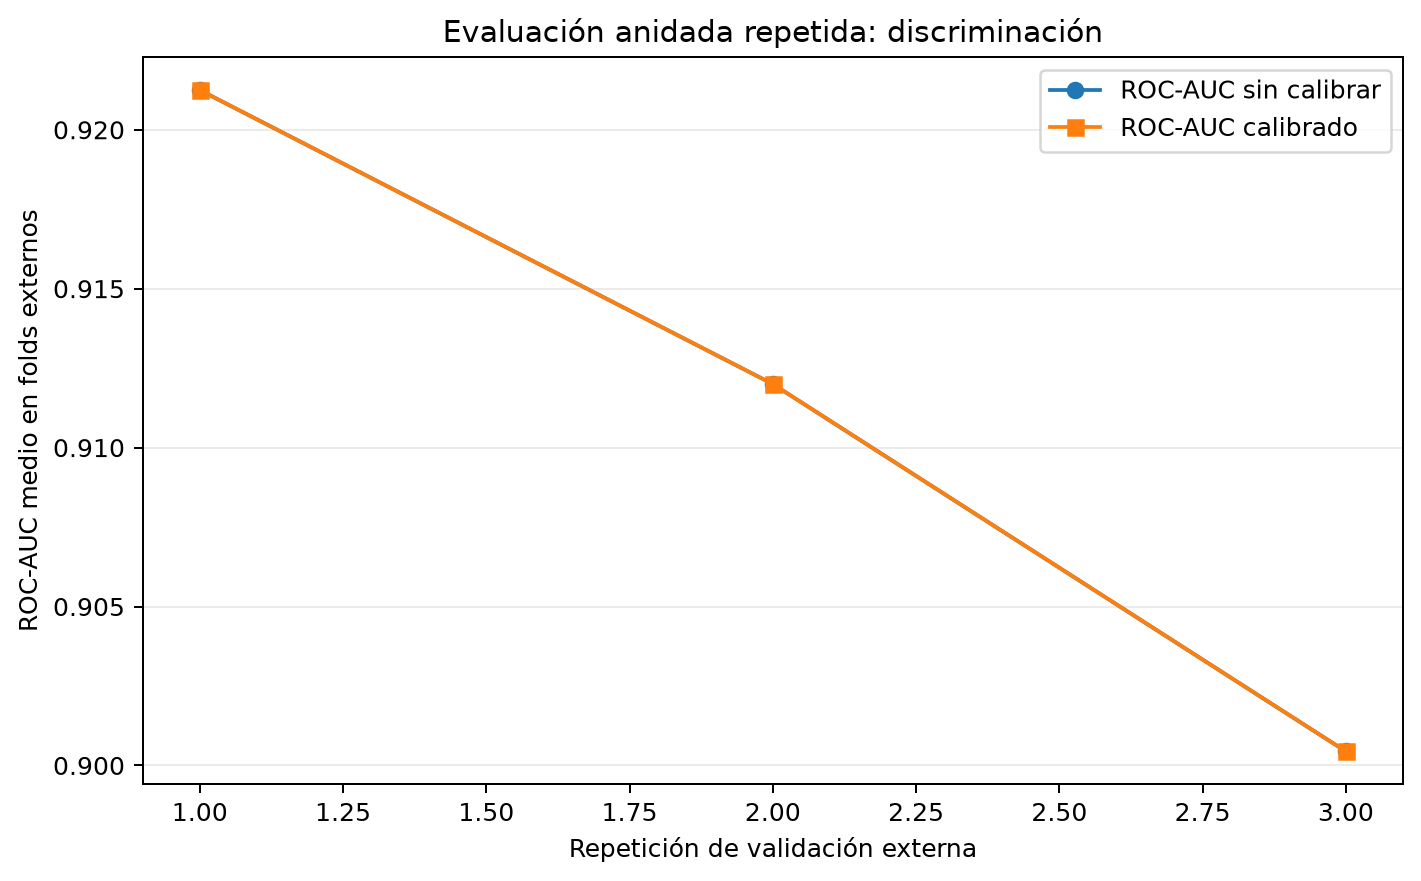
\includegraphics[width=0.9\textwidth]{../outputs/figures/nested_cv_roc_auc_repeticiones.png}
  \caption{ROC-AUC por repetición externa en la evaluación anidada. La calibración sigmoide no cambia el orden de scores.}
  \label{fig:nested-auc}
\end{figure}

\begin{figure}[H]
  \centering
  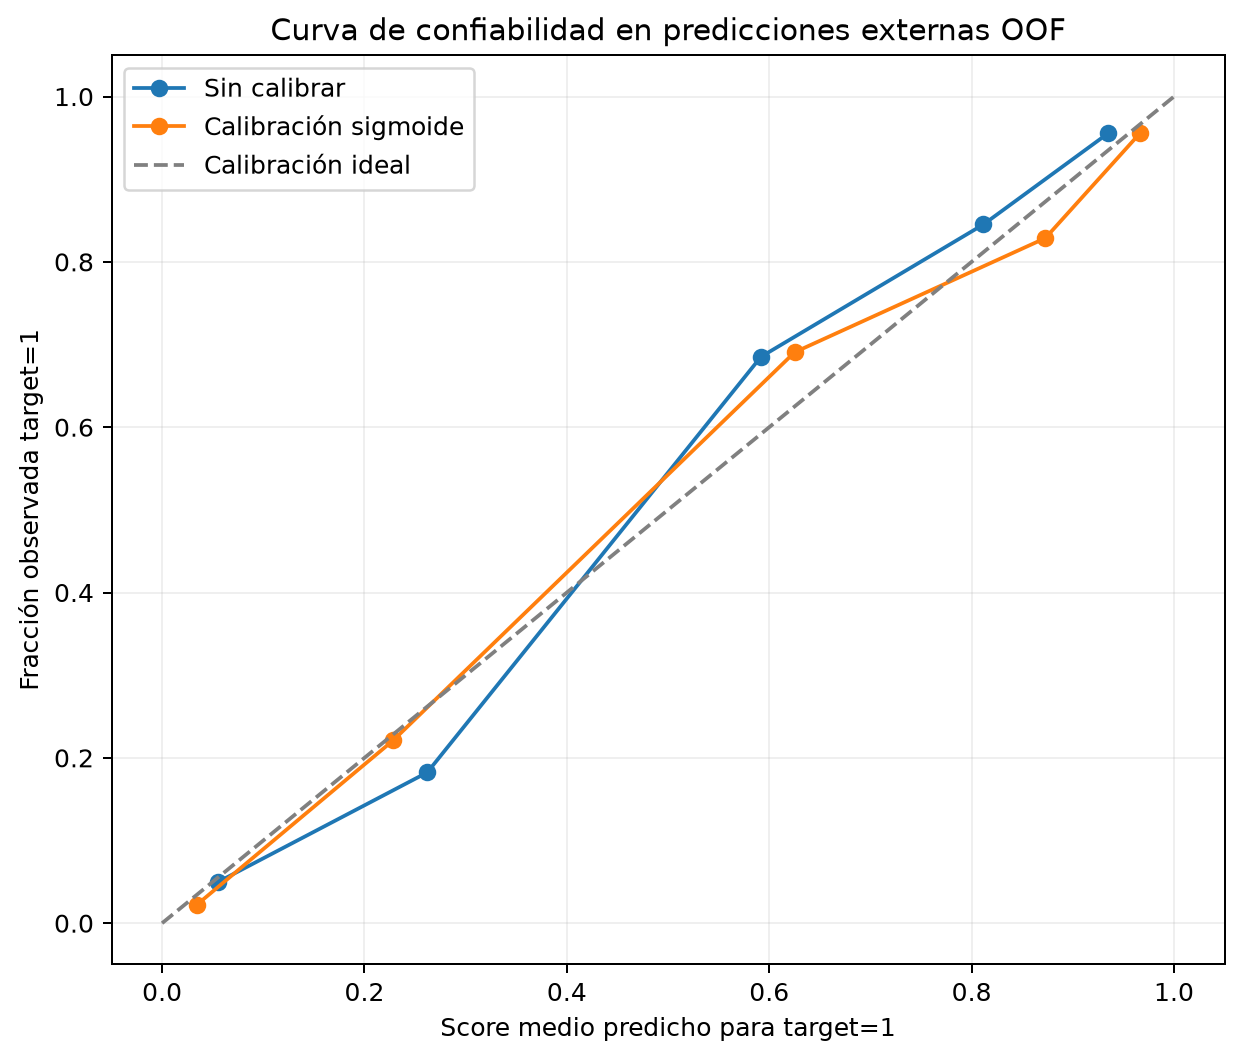
\includegraphics[width=0.9\textwidth]{../outputs/figures/nested_cv_calibracion.png}
  \caption{Curvas de calibración agregadas sobre predicciones externas; Brier y log-loss resumen el error probabilístico.}
  \label{fig:nested-calibracion}
\end{figure}

\begin{figure}[H]
  \centering
  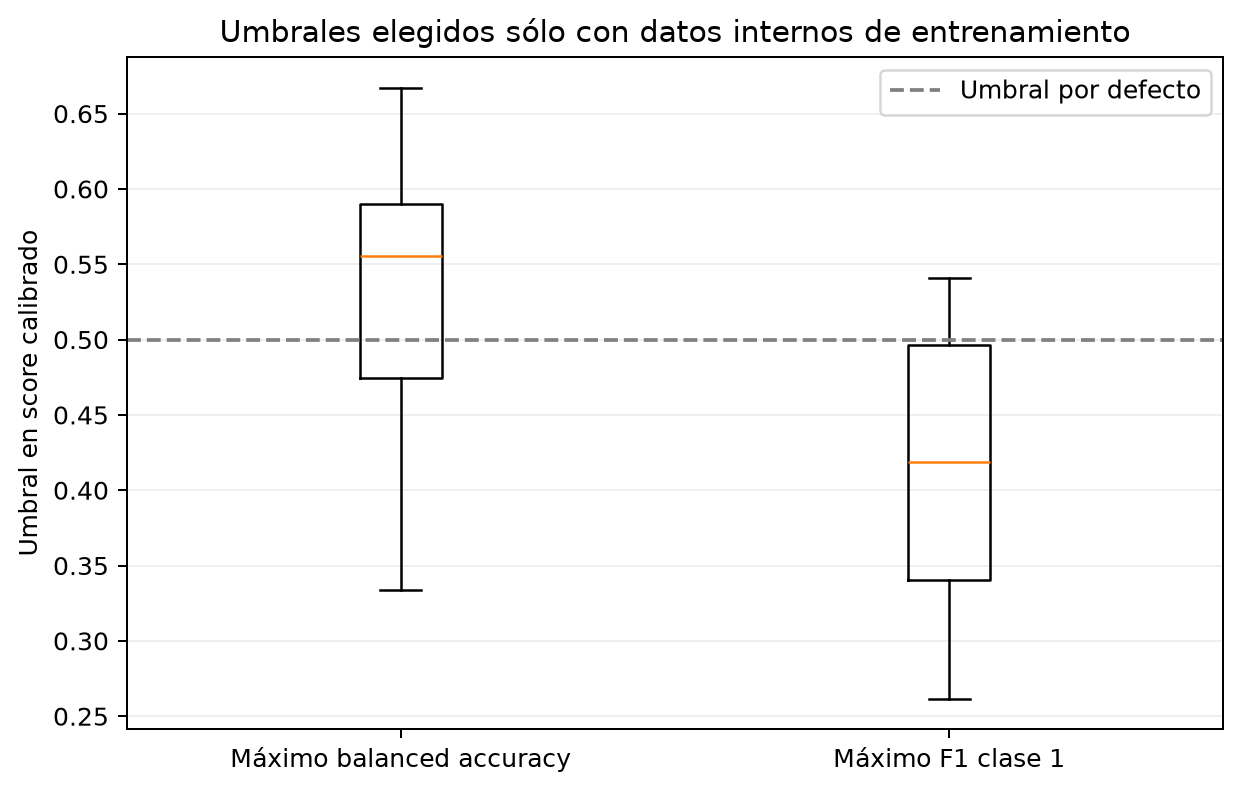
\includegraphics[width=0.9\textwidth]{../outputs/figures/nested_cv_umbral.png}
  \caption{Umbrales seleccionados dentro de entrenamiento externo. Su dispersión no determina un umbral clínico.}
  \label{fig:nested-umbrales}
\end{figure}

La ficha del proveedor Kaggle declara $0$ como sin enfermedad y $1$ como enfermedad; se utiliza esa definición para orientar métricas por clase, pero no se validó clínicamente ni se trazaron los registros a UCI. No hay cohorte externa independiente, autorizada y compatible en el repositorio. Por ello, los resultados son internos y no miden desempeño esperado en una población clínica. El notebook reproducible, la auditoría de fuente y las tablas se describen en \texttt{docs/evaluacion\_modelo\_robusta.md}.

\section{Interpretación, limitaciones y uso}
Los valores son resultados experimentales de un conjunto académico con 302 observaciones únicas. La copia de datos contiene duplicación extensa, hay diferencias de dominio pendientes de aclarar y no se conoce población de referencia. El ROC-AUC de prueba de 0,875 y las demás métricas describen una partición; la evaluación anidada ofrece una estimación interna adicional. Ninguna constituye desempeño clínico esperado. La calibración sigmoide se evaluó experimentalmente, pero no se liberó como score clínico ni se validó externamente.

Se incluyen atribuciones TreeSHAP globales y locales para explicar este artefacto XGBoost; éstas describen la lógica del modelo y no prueban causalidad, equidad ni importancia clínica. La auditoría de desempeño por subgrupos sigue siendo insuficiente. No hay datos hospitalarios, aprobación institucional, revisión clínica, servicio/API, despliegue productivo ni monitoreo. La inferencia batch local está demostrada sólo con cinco casos sintéticos y no modifica ni reentrena el artefacto.

\section{Reproducción y artefactos}
El código fuente de entrenamiento se encuentra en \texttt{src/modeling.py}; el desarrollo y las figuras se documentan en el notebook técnico. El entorno de dependencias está fijado mediante \texttt{uv.lock}. El modelo serializado está en \texttt{outputs/models/heart\_disease\_pipeline.joblib}; su uso requiere las dependencias y el esquema de entrada documentado. Los gráficos incluidos en este informe se generan bajo \texttt{outputs/figures/}; las tablas de auditoría y métricas, bajo \texttt{outputs/tables/}.

Para instalar el entorno y ejecutar el análisis desde la raíz del repositorio:
\begin{lstlisting}[language=bash]
uv sync
uv run jupyter lab notebooks/04_implementacion_tecnica_3_1_2.ipynb
\end{lstlisting}

La documentación del preprocesamiento sigue prácticas de ajuste de transformadores dentro de los datos de entrenamiento para evitar fuga de información \parencite{scikit-learn-common-pitfalls}. La documentación del conjunto de origen está referenciada como contexto de procedencia, no como validación de esta copia \parencite{uci-heart-disease,kaggle-heart}.

\printbibliography
\end{document}
